\documentclass[lettersize,journal]{IEEEtran}
\usepackage[T1]{fontenc}
\usepackage{amsmath,amsfonts}
\usepackage{algpseudocode}
\usepackage{algorithm}
\usepackage{array}
\usepackage{booktabs}
\usepackage[caption=false,font=normalsize,labelfont=sf,textfont=sf]{subfig}
\usepackage{textcomp}
\usepackage{stfloats}
\usepackage{url}
\usepackage{verbatim}
\usepackage{graphicx}
\usepackage{cite}
\hyphenation{op-tical net-works semi-conduc-tor IEEE-Xplore}

\usepackage{amssymb}
\usepackage{amsthm}
\usepackage{xcolor}
\usepackage{pgfplots}
\pgfplotsset{compat=1.18}
\pgfplotsset{auditaxis/.style={
 width=0.98\linewidth,height=0.76\linewidth,scale only axis=false,
 font=\sffamily\scriptsize,
 tick label style={font=\sffamily\scriptsize,/pgf/number format/fixed,/pgf/number format/precision=2,/pgf/number format/1000 sep={}},
 label style={font=\sffamily\small},tick align=outside,
 axis x line*=bottom,axis y line*=left,
 tick style={black!45,line width=0.35pt},axis line style={black!50,line width=0.45pt},
 scaled ticks=false,xminorticks=false,yminorticks=false,
 enlarge x limits=0.12,enlarge y limits={upper,value=0.15},
 xmajorgrids=false,ymajorgrids=true,grid style={draw=black!10,line width=0.25pt},
 axis background/.style={fill=white},clip mode=individual}}
\usepackage[colorlinks=true,linkcolor=blue,citecolor=blue,urlcolor=blue]{hyperref}

\newtheorem{assumption}{Assumption}
\newtheorem{theorem}{Theorem}
\newtheorem{lemma}{Lemma}
\newtheorem{remark}{Remark}
\newtheorem{proposition}{Proposition}

\newcommand{\ZZ}{\mathbb{Z}}
\newcommand{\GG}{\mathbb{G}}
\newcommand{\FF}{\mathbb{F}}
\newcommand{\CompExp}{\mathcal{E}}
\newcommand{\CompPair}{\mathcal{P}}
\newcommand{\CompField}{\mathcal{F}}
\newcommand{\ComField}{\CompField}

\newcommand{\dleq}{\mathsf{DLEQ}}
\newcommand{\dleqvrf}{\mathsf{DLEQVrf}}

\newcommand{\vssreshare}{\mathsf{VSS.ReShare}}
\newcommand{\vssaggregate}{\mathsf{VSS.ReshareAgg}}
\newcommand{\vssrerec}{\mathsf{VSS.ReshareRec}}

\newcommand{\vssshare}{\mathsf{VSS.Share}}
\newcommand{\vssvrf}{\mathsf{VSS.Verify}}
\newcommand{\vssrec}{\mathsf{VSS.Reconstruct}}

\newcommand{\DKGGenPK}{\mathsf{DKG.GenPK}}
\newcommand{\DKGGenSK}{\mathsf{DKG.GenSK}}

\newcommand{\blssetup}{\mathsf{BLS.Setup}}
\newcommand{\blskeygen}{\mathsf{BLS.KeyGen}}
\newcommand{\blssign}{\mathsf{BLS.Sign}}
\newcommand{\blsvrf}{\mathsf{BLS.Verify}}
\newcommand{\blscombine}{\mathsf{BLS.Combine}}
\newcommand{\blsbatch}{\mathsf{BLS.Batch}}
\newcommand{\blsbatchvrf}{\mathsf{BLS.BatchVrf}}

\newcommand{\pssetup}{\mathsf{PS.Setup}}
\newcommand{\pskeygen}{\mathsf{PS.Kengen}}
\newcommand{\psPrepareBlindSign}{\mathsf{PS.PrepareBlindSign}}
\newcommand{\psBlindSign}{\mathsf{PS.BlindSign}}
\newcommand{\psUnblind}{\mathsf{PS.Unblind}}
\newcommand{\psSign}{\mathsf{PS.Sign}}
\newcommand{\psobtaincred}{\mathsf{PS.ObtainCred}}
\newcommand{\psgentoken}{\mathsf{PS.GenToken}}
\newcommand{\psver}{\mathsf{PS.Verify}}

\newcommand{\dacsetup}{\mathsf{DAC.Setup}}
\newcommand{\dacevolve}{\mathsf{DAC.Evolve}}
\newcommand{\dackeygen}{\mathsf{DAC.Kengen}}
\newcommand{\dacPrepareBlindSign}{\mathsf{DAC.PrepareBlindSign}}
\newcommand{\dacBlindSign}{\mathsf{DAC.BlindSign}}
\newcommand{\dacobtaincred}{\mathsf{DAC.ObtainCred}}
\newcommand{\dacgentoken}{\mathsf{DAC.GenToken}}
\newcommand{\dacver}{\mathsf{DAC.VerifyTok}}
\newcommand{\dactrace}{\mathsf{DAC.Trace}}

\newcommand{\dacadd}{\mathsf{DAC.AddAttr}}
\newcommand{\dacupdate}{\mathsf{DAC.UpdateAttr}}
\newcommand{\dacremeove}{\mathsf{DAC.RemoveAttr}}
\newcommand{\dacquerry}{\mathsf{DAC.QueryAttr}}

\newcommand{\RDKGGenPK}{\mathsf{RDKG.GenPK}}
\newcommand{\RDKGEvolve}{\mathsf{RDKG.Evolve}}
\newcommand{\RDKGGenSK}{\mathsf{RDKG.GenSK}}

\newcommand{\SK}{\mathsf{SK}}
\newcommand{\PK}{\mathsf{PK}}
\newcommand{\PP}{\mathsf{PP}}

\newcommand{\SA}{\mathsf{SA}}
\newcommand{\SAGetPub}{\mathsf{SA.GetPub}}
\newcommand{\SAGetPriv}{\mathsf{SA.GetPriv}}
\newcommand{\SApk}{\mathbf{PK}}
\newcommand{\SAsk}{\mathbf{SK}}
\newcommand{\SAr}{\mathbf{R}}
\newcommand{\Fp}{\FF_p}
\newcommand{\GOne}{G_1}
\newcommand{\GTwo}{G_2}
\newcommand{\GT}{G_T}
\newcommand{\pair}{e}

\newcommand{\SRS}{\mathsf{SRS}}

\newcommand{\Setup}{\mathsf{Setup}}
\newcommand{\Store}{\mathsf{Store}}
\newcommand{\Chal}{\mathsf{Challenge}}
\newcommand{\ProofGen}{\mathsf{ProofGen}}
\newcommand{\Verify}{\mathsf{Verify}}

\definecolor{ZhangTPDS23}{HTML}{228877}
\definecolor{MiaoSCIS2026}{HTML}{AA5588}
\definecolor{XuTIFS26}{HTML}{DD9933}
\definecolor{MultiAudit}{HTML}{3366AA}

\definecolor{YuTC25}{HTML}{889933}
\begin{document}

\title{MultiAudit: Efficient Multi-File Integrity Auditing for Mobile Cloud Storage}

\author{Liang Zhang,~\IEEEmembership{Member,~IEEE}, Xuyan Wei, Borui Chen, Haibin Kan,~\IEEEmembership{Member,~IEEE,} and Jiheng Zhang
\thanks{Liang Zhang and Jiheng Zhang are with Department of Industrial Engineering and Decision Analytics, Hong Kong University of Science and Technology, Clear Water Bay, Kowloon, Hong Kong. (e-mail: scottzhang@ust.hk; jiheng@ust.hk); Xuyan Wei is with School of Cyberspace Security (School of Cryptology), Hainan University, Haikou, 570228, China. (e-mail: wxy233@hainanu.edu.cn); Borui Chen and Haibin Kan are with College of Computer Science and Artificial Intelligence, Fudan University, Shanghai 200433, China. Haibin Kan is also with Shanghai Engineering Research Center of Blockchain, Shanghai 200433, China and Shanghai Institute for Mathematics and Interdisciplinary Sciences, Shanghai, 200433, China.(e-mail: 23210240072@m.fudan.edu.cn; hbkan@fudan.edu.cn;)}

\thanks{*Corresponding authors: Haibin Kan and Jiheng Zhang.}
}

\maketitle
\begin{abstract}
Multi-file integrity auditing must authenticate sampled tags and verify data-dependent opening claims without retrieving entire files. We present MultiAudit, a PDP-oriented construction combining per-file compact Merkle multiproofs (CMMs) with a two-witness batch opening protocol. CMMs remove duplicated authentication hashes; batched KZG openings aggregate quotient coefficients before commitment, reducing the data witnesses to two group elements for an audit batch sharing one data SRS. Distinct file-specific evaluation points and a two-stage Fiat--Shamir transcript bind the batch opening statements. Independent file roots retain file addition and active audit-set removal without rebuilding surviving files' authentication state. We establish correctness, public verifiability, marginal evaluation-masking privacy, and batch-opening soundness under explicitly stated algebraic-group and random-oracle assumptions. Fresh scalar masks and Schnorr proofs do not prevent public candidate testing of evaluation group encodings; neither general data possession nor sector confidentiality is established. We compare group-operation and communication costs with representative auditing protocols under explicit counting and encoding conventions. For $(m,B,s,c)=(40,10\,\mathrm{MB},80,690)$, MultiAudit achieves measured proof-generation and verification speedups of 2.78$\times$ and 5.56$\times$ relative to Zhang et al.~\cite{ZhangTPDS23}; its mean encoded response is 71.9\% smaller than the native payload accounting of Xu et al.~\cite{XuTIFS26}. A physical iPhone~13 client performs owner Store and optional verification; complete local verification, including decoding and interface overhead, is 23.6\% and 42.3\% faster than Xu et al.~\cite{XuTIFS26} and Yu et al.~\cite{YuTC25} for ten files.
\end{abstract}

\begin{IEEEkeywords}
Provable Data Possession, Data Integrity Auditing, KZG Commitments, Multi-File Auditing
\end{IEEEkeywords}

\section{Introduction}

Personal photographs, documents, and application records increasingly reside in cloud storage accessed from mobile devices. These files can have lasting personal value, making their integrity an essential aspect of personal data security. Once a local copy is removed, unnoticed corruption, incomplete storage, or an incorrect response from a cloud service can be difficult for the owner to detect. Encryption addresses confidentiality but does not by itself provide an efficient remote integrity check. The provable data possession (PDP) model of Ateniese et al.~\cite{Ateniese2007PDP} enables probabilistic checking of outsourced data through challenges and authenticators, avoiding retrieval of entire files for every audit. This capability is particularly useful for personal storage collections that remain in the cloud for extended periods.

Mobile devices are routine endpoints for creating, editing, and sharing these collections. A user may process many independently managed files while sharing the device's computation, memory, battery, and network resources with other applications. Dinh et al.~\cite{Dinh2013MCC} identify these resource constraints as central considerations in mobile cloud computing. An audit must therefore account for the server's proof-generation work, the response transmitted to the verifier, and verification on the client. Public verification also allows the owner to delegate checking to an authorized service without sharing a verification secret. Offloaded auditing for resource-constrained devices is explored by Li et al.~\cite{Li2015OPoR}, while Yu et al.~\cite{Yu2022Offline} investigate offline auditing for vehicular clouds. Whether verification is local or delegated, the audit must use current owner-authenticated metadata and accommodate file addition and removal without rebuilding unrelated files' authentication state.

For recent auditing constructions that explicitly authenticate sampled tags, including those of Xu et al.~\cite{XuTIFS26} and Yu et al.~\cite{YuTC25}, it is useful to distinguish two layers. The \emph{tag-commitment layer} authenticates the ordered tag collection and the positions of sampled tags. The \emph{data-consistency layer} checks that returned data-dependent evaluation claims agree with those authenticated tags. Functionally, the first layer commits to a vector of tags with position binding. It can use a Merkle root or an algebraic vector commitment; the second layer can use polynomial commitments to verify the evaluation relations. These are complementary roles, and a polynomial commitment used for data tags does not itself establish their membership in the owner's current file.

The choice of the first-layer mechanism creates a computation--communication trade-off. Merkle authentication~\cite{Merkle1988} relies on collision-resistant hashing, needs no algebraic trusted setup, and authenticates one position with a logarithmic-length path. Its drawback is the repeated transmission of sibling hashes when many such paths overlap. Succinct vector commitments~\cite{Catalano2013VC,Campanelli20ASIACRYPT} can provide short position openings; polynomial commitments such as KZG~\cite{Kate2010KZG} can support vector authentication after suitable field encoding and binding of positions. KZG offers constant-size opening witnesses, but entails structured public parameters and algebraic proof generation and verification. Consequently, replacing a Merkle structure with an algebraic commitment changes setup, encoding, and computation requirements as well as proof size. We retain independent hash-based file roots and reduce their authentication traffic within that layout.

To address the first layer, we use the compact Merkle multiproofs (CMMs) of Ramabaja and Avdullahu~\cite{Ramabaja2020Compact}. Instead of returning a separate membership path for each challenged tag, the server supplies one CMM per file. Overlapping branches share intermediate computations, and each required auxiliary subtree hash is transmitted once in a canonical traversal order. The queried indices determine its position and orientation, eliminating separate auxiliary position labels. This removes duplicated authentication hashes and reduces the response component that grows with the challenged set. Each file retains its own root, so adding a file or removing it from the active audit set leaves the surviving files' authentication state intact. The response still includes sampled tags and a challenge-dependent number of auxiliary hashes.

The second layer presents a different bottleneck: constructing an opening commitment independently for every file repeats group operations across the audit batch. For example, the witness-generation term of Xu et al.~\cite{XuTIFS26} grows as $m(s-1)\CompExp$, where $m$ is the number of files and $s$ the sectors per chunk. We address this cost by instantiating the two-witness batch-opening construction of Boneh et al.~\cite[Sec.~4.1]{Boneh2020PCS}. The server first forms the file-specific quotient polynomials, aggregates their coefficients over the field, and then commits to two aggregate quotients. Together with the per-file mask commitments, this gives $[2(s-1)+2m]\CompExp$ scalar terms. Challenged-data aggregation still requires $\mathcal O(mcs)$ field work, where $c$ is the challenged-chunk count. Constant-response designs such as that of Zhang et al.~\cite{ZhangTPDS23} remain important alternatives; our objective is to reduce proof-generation work together with authentication traffic in the chosen two-layer layout.

Combining these reductions requires binding the two layers correctly. Files use distinct evaluation points, so directly adding their data polynomials does not produce one evaluation statement at a common point. The batch check must instead preserve each authenticated tag collection's relation to its file-specific claim. Moreover, the transcript must bind the current roots, file order, challenge, sampled tags, and masked evaluations before deriving the corresponding random challenges. MultiAudit fixes the first aggregate witness before deriving the second challenge. A batch shares one data structured reference string (SRS), while independent file roots preserve file-level management; files using different data SRS identifiers require separate batches. These requirements determine the challenge ordering and transcript of our construction.

We present \textbf{MultiAudit} with these two complementary reductions and explicit security boundaries. Public parameters and the current owner-authenticated registry suffice for verification, enabling local or authorized delegated checking. Fresh scalar masks and transcript-bound Schnorr proofs~\cite{Schnorr1991Sig} provide marginal evaluation masking. Privacy against an auditor, studied by Wang et al.~\cite{Wang2013TC}, also requires considering the complete response: MultiAudit's public evaluation group encodings permit candidate testing, so full-transcript confidentiality is not claimed. We establish correctness, public verifiability, and conditional soundness of authenticated batch openings under stated algebraic-group and random-oracle assumptions. Sampling coverage is analyzed separately from general data possession or retrievability.

Our evaluation combines complete protocol calls under a common native backend with a physical-iPhone client and single-file EVM verification. At 40 files of 10~MB each and 80 sectors per chunk, MultiAudit provides proof-generation and verification speedups of 2.78$\times$ and 5.56$\times$ relative to Zhang et al.~\cite{ZhangTPDS23}. Its mean encoded response, including framing, is 71.9\% smaller than the native payload accounting of Xu et al.~\cite{XuTIFS26}, excluding framing. The constant-response advantages of Zhang et al.~\cite{ZhangTPDS23} and Miao et al.~\cite{MiaoSCIS2026} remain explicit. The iPhone~13 experiment places Store on the owner, leaves ProofGen in the cloud, and measures optional local verification for ten files. A separate single-file EVM experiment evaluates complete verification gas. These measurements distinguish native protocol work, client interface overhead, and serialized uploads; battery energy and wide-area wireless conditions are outside the evaluation.

The main contributions are as follows.
\begin{itemize}
\item \textbf{Compact authentication for independently managed files.} We integrate per-file CMMs into multi-file auditing to remove duplicated path hashes while preserving owner-authenticated roots and file addition/removal. Canonical encoding and traversal bind sampled tags to their file positions.
\item \textbf{Reduced batch proof-generation work.} We instantiate two-witness KZG batch openings by aggregating quotient coefficients before commitment. Distinct file-specific points, a common data SRS, and explicitly ordered transcript challenges link the authenticated tags to the batch relation.
\item \textbf{Security and cost characterization.} We establish correctness, public verifiability, marginal evaluation-masking privacy, and conditional authenticated-opening soundness. We characterize remaining transcript leakage and account separately for group operations, polynomial field work, and auxiliary hashes.
\item \textbf{Implementation and evaluation.} We compare complete calls and response sizes with four published constructions under a common backend. A physical iPhone~13 client measures owner Store computation and uploads, together with optional local verification, against Xu et al.~\cite{XuTIFS26} and Yu et al.~\cite{YuTC25}; a separate EVM experiment compares single-file verification gas. The comparison retains each native construction and sampling convention.
\end{itemize}

\section{Preliminaries}
\label{sec:preliminaries}
For an integer $t\geq1$, write $[t]=\{1,\ldots,t\}$. Let $\lambda$ be the security parameter; PPT and $\mathsf{negl}(\lambda)$ denote probabilistic polynomial time and a negligible function, respectively. We use canonical, injective, length-framed encodings $\mathsf{enc}$ for tuples, indices, and group elements. Concatenations below use this framing, with distinct literal domain labels. All indexed collections are ordered sequences; finite-set sampling is uniform unless stated otherwise.

\subsection{Compact Merkle Multiproofs (CMMs)}
\label{subsec:multiproofs}
Merkle trees~\cite{Merkle1988} authenticate an ordered collection through a trusted root hash. Proving membership of several values with separate paths repeats hashes wherever the paths overlap. A CMM~\cite{Ramabaja2020Compact} merges these paths and supplies each required sibling hash once. Its positions and left/right orientation follow from the queried indices, so no auxiliary position labels are needed.

Let $H_1:\{0,1\}^*\to\{0,1\}^{\lambda}$ be a hash function. For $n\geq1$ values $(X_j)_{j=1}^n$ and a namespace identifier $\mathsf{id}\in\{0,1\}^*$, the leaf at position $j\in[n]$ is $L_j=H_1(\mathsf{leaf}\|\mathsf{id}\|j\|\mathsf{enc}(X_j)).$
An internal node with left and right child hashes $u,v$ has hash $H_1(\mathsf{node}\|u\|v)$. The complete binary tree has height $L=\lceil\log_2 n\rceil$. Positions at leaf $n<j\leq2^L$ are padded by $H_1(\mathsf{pad}\|\mathsf{id}\|n\|j)$. The labels $\mathsf{leaf}$, $\mathsf{node}$, and $\mathsf{pad}$ provide domain separation. Verification uses the trusted root $\Gamma$ and metadata $(\mathsf{id},n)$.

Let $J\subseteq[n]$ contain $c\geq1$ queried indices, listed in increasing order, and let $\mathcal A(J)$ be the ordered list of auxiliary hashes. Starting from the queried leaves, the prover processes one level at a time toward the root, with touched parents ordered from left to right. At each parent, it combines both known children, or appends the missing sibling hash to $\mathcal A(J)$ before combining. Missing siblings are transmitted even for fully padded subtrees. The verifier requires one value per queried index and $\lambda$-bit auxiliary hashes, hashes the supplied values, and repeats this traversal in the same order. It rejects malformed encodings, unordered, repeated, or out-of-range indices, missing or unused hashes, or a reconstructed root unequal to $\Gamma$.

The number of transmitted auxiliary hashes satisfies
\begin{equation}\label{eq:aux_count}
|\mathcal A(J)|\leq cL.
\end{equation}
Root reconstruction hashes $c$ real leaves and $|\mathcal A(J)|+c-1$ internal nodes: the reconstructed binary tree has $c+|\mathcal A(J)|$ terminal nodes, comprising the queried leaves and auxiliary subtree roots.

\begin{assumption}[Collision Resistance]\label{ass:hash}
Every PPT adversary produces distinct inputs $x\ne x'$ with $H_1(x)=H_1(x')$ with probability at most $\mathsf{negl}(\lambda)$.
\end{assumption}

\subsection{Polynomial Basics}
\label{subsec:polynomial_basics}
Polynomial division characterizes evaluation claims, while polynomial root bounds~\cite{Schwartz1980} control the probability of a false identity holding at a random point. Let $\FF_p$ be the field of prime order $p$. For $d\geq1$, write $\FF_p^{<d}[X]$ for univariate polynomials over $\FF_p$ of degree less than $d$, including zero, with the convention $\deg0=-\infty$. All polynomial identities are over $\FF_p[X]$, and all group exponents are interpreted modulo $p$.

For $F(X)\in\FF_p[X]$ and $r,u\in\FF_p$, polynomial division gives a unique quotient $q(X)$ such that $F(X)-u=(X-r)q(X)+F(r)-u$. Hence $X-r$ divides $F(X)-u$ exactly when $u=F(r)$, and $\deg q\leq\deg F-1$.

\begin{lemma}[Univariate Schwartz--Zippel]\label{lem:schwartz_zippel}
Let $P(X)\in\FF_p[X]$ be a nonzero polynomial of degree at most $d\geq0$. It has at most $d$ roots in $\FF_p$. For any nonempty $S\subseteq\FF_p$, if $P$ and $S$ are fixed before $r$ is sampled uniformly from $S$, then $\Pr[P(r)=0]\leq\min\{1,d/|S|\}$. In particular, sampling from $\FF_p$ gives the bound $d/p$.
\end{lemma}

\subsection{Batched KZG Openings}
\label{subsec:batch_openings}
A KZG commitment binds a polynomial to one group element and supports verification of its value at a chosen point~\cite{Kate2010KZG}. Verifying several openings separately requires one witness per claim. The two-witness batch-opening construction of Boneh et al.~\cite[Sec.~4.1]{Boneh2020PCS} combines claims at distinct points under a common structured reference string (SRS), using two successive challenges and one pairing equation.

Let $(\GG_1,\GG_2,\GG_T)$ be groups of order $p$, with generators $g\in\GG_1$, $h\in\GG_2$, and a nondegenerate, efficiently computable bilinear map $e:\GG_1\times\GG_2\to\GG_T$. For degree bound $2\leq s<p$, setup samples $\tau\in\FF_p$ uniformly, keeps it hidden from the prover and verifier, and publishes $\SRS=(g,g^\tau,\ldots,g^{\tau^{s-1}},h,h^\tau)$. For $F(X)=\sum_{k=0}^{s-1}a_kX^k$, its commitment is $g^{F(\tau)}=\prod_{k=0}^{s-1}(g^{\tau^k})^{a_k}$. Thus commitments are computable from the public SRS without knowing $\tau$. We use exponent notation throughout. Homomorphism gives $g^{aF(\tau)+bG(\tau)}=(g^{F(\tau)})^a(g^{G(\tau)})^b$ for $a,b\in\FF_p$ and $F,G\in\FF_p^{<s}[X]$.

The batch statement is $(B_i,r_i,u_i)_{i=1}^m$, where $1\leq m<p$, $B_i=g^{P_i(\tau)}\in\GG_1$, $P_i\in\FF_p^{<s}[X]$, $r_i,u_i\in\FF_p$, and the $r_i$ are distinct. For honest claims $u_i=P_i(r_i)$, polynomial division in Section~\ref{subsec:polynomial_basics} gives $q_i(X)=(P_i(X)-u_i)/(X-r_i)$. After fixing the statement, sample $\gamma$ uniformly from $\FF_p^*$ and send $C_Q=g^{Q(\tau)}$, where $Q=\sum_i\gamma^{i-1}q_i$. Only after fixing $C_Q$, sample $z$ uniformly from $\FF_p\setminus\{r_i\}_{i=1}^m$ and send $C_W=g^{W(\tau)}$, where $W=\sum_i\beta_iq_i$ and $\beta_i=\gamma^{i-1}/(z-r_i)$. Honest $q_i,Q,W$ have degree at most $s-2$. The proof $(C_Q,C_W)\in\GG_1^2$ is accepted exactly when
\begin{equation}\label{eq:batch_opening_interface}
\begin{aligned}
D=C_Q^{-1}\prod_{i=1}^m(B_i g^{-u_i})^{\beta_i},\\
e(D\cdot C_W^z,h)=e(C_W,h^\tau).
\end{aligned}
\end{equation}

\begin{assumption}[Algebraic Reduction for Batched Openings]\label{ass:batch_opening_agm}
For the honestly generated common SRS, work in the algebraic group model~\cite{Fuchsbauer2018AGM} and assume the batched-KZG reduction of Boneh et al.~\cite[Sec.~4.1]{Boneh2020PCS}: an algebraic adversary supplies representations of output group elements in previously available elements. Except with negligible reduction failure probability $\varepsilon_{\rm alg}(\lambda)$, these representations determine a polynomial $Q\in\FF_p^{<s}[X]$ fixed before $z$, and accepting Equation~\eqref{eq:batch_opening_interface} implies $G_z(z)=0$, where $G_z(X)=\sum_i\beta_i(P_i(X)-u_i)-Q(X)$. The input polynomials $P_i$ are fixed with the statement.
\end{assumption}

\subsection{Schnorr Proofs of Knowledge}
\label{subsec:schnorr}
For a public $Y=g^x\in\GG_1$, Schnorr~\cite{Schnorr1991Sig} proves knowledge of $x\in\FF_p$. We apply the Fiat--Shamir transform~\cite{FiatShamir1987} to derive the challenge from the public transcript. With public context $\mathsf{ctx}$, sample fresh $t\leftarrow\FF_p$, set $A=g^t$, derive $\chi=H_{2,\mathsf d}(\mathsf{ctx},Y,A)\in\FF_p$ under a fixed proof domain $\mathsf d$, and respond with $\zeta=t+\chi x$. The proof $(A,\zeta)\in\GG_1\times\FF_p$ is accepted if $g^\zeta=AY^\chi$. The symbol $\zeta$ denotes a Schnorr response; $z$ above denotes the batch opening's second challenge.

\begin{assumption}[Fiat--Shamir Model]\label{ass:random_oracle}
$H_2$ is a domain-separated random oracle~\cite{BellareRogaway1993}. The notation $H_{2,\mathsf d}$ denotes hash-to-field under domain $\mathsf d$, with counter-based rejection sampling uniform on the prescribed nonempty subset of $\FF_p$. Distinct domains are independent.
\end{assumption}
\begin{assumption}[Schnorr Knowledge Soundness]\label{ass:schnorr_knowledge}
Fiat--Shamir Schnorr proofs for the relation $\{(Y,x):Y=g^x\}$ are knowledge-sound in this model, with the full public context bound into the challenge.
\end{assumption}

\section{System Model and Security Model}

\subsection{System Model}
\paragraph{System Entities}
We consider a PDP-oriented multi-file auditing architecture comprising three entities: a Data Owner (DO), a Cloud Server (CS), and a Verifier (V).
\begin{itemize}
    \item \textbf{Data Owner}: The DO outsources a set of $m$ files to the CS for long-term storage. To ensure data integrity without maintaining local copies, the DO delegates periodic auditing to the V.
    \item \textbf{Cloud Server}: The CS is modeled as untrusted and computationally bounded: it may delete, corrupt, or selectively withhold files or chunks to save storage or bandwidth.
    \item \textbf{Verifier}: The V is honest-but-curious. It executes the auditing protocol faithfully but may attempt to infer sensitive information from audit transcripts.
\end{itemize}

\paragraph{File Representation}
A file is divided into multiple chunks, and each \textbf{chunk} can be represented through polynomial coefficients. Each coefficient is referred to as a \textbf{sector}.
Let $m$ denote the number of files in one audit workload, $n$ the number of chunks per file, and $s$ the number of sectors per chunk. Native multi-file batch verification combines the main file-specific algebraic relations into one aggregated relation; repeating a single-file verifier $m$ times does not provide this capability. Each chunk is parsed into $s$ field elements from $\FF_p$ and algebraically encoded as a polynomial of degree at most $s-1$:
$$
    f_{i,j}(X) = \sum_{k=0}^{s-1} m_{i,j,k} X^k, \quad i \in [m], \; j \in [n],
$$
where $m_{i,j,k}$ represents the $k$-th sector of the $j$-th chunk in file $i$.
A \textbf{tag} is used to represent the \(j\)-th chunk through a KZG polynomial commitment, i.e., $\sigma_{i,j} =  g^{f_{i,j}(\tau)} \in \GG_1$. Further, tags of each file are organized into a Merkle tree to guarantee correct indexing and membership. Each file has an independent Merkle root. Every file in one opening batch must use the same data SRS (including generators, trapdoor powers, and degree bound). Files with different SRS identifiers require separate opening batches.

Table~\ref{tab:notation} collects the protocol-specific symbols used in the system model and construction.

\begin{table}[htbp]
\centering
\caption{Summary of Notation and System Parameters}
\label{tab:notation}
\begin{tabular}{@{} p{0.065\textwidth} p{0.385\textwidth} @{}}
\hline
\textbf{Symbol} & \textbf{Description} \\
\hline
$\lambda$ & Security parameter. \\
$p$ & Prime order of $\FF_p$ and $(\GG_1, \GG_2, \GG_T)$. \\
$\FF_p^{<d}[X]$ & Polynomials over $\FF_p$ with degree less than $d$. \\
$g, h$ & Public generators of $\GG_1$ and $\GG_2$, respectively. \\
$e(\cdot, \cdot)$ & Bilinear map $e: \GG_1 \times \GG_2 \to \GG_T$. \\
$\tau$ & Secret trapdoor used for the structured reference string. \\
$\SRS$ & Public parameters $(g, g^\tau, \dots, g^{\tau^{s-1}}, h, h^\tau)$ supporting polynomial degrees $< s$. \\
$H_1$ & Hash function for Merkle tree construction. \\
$H_2$ & Fiat--Shamir random oracle for challenge derivation. \\
$m, n, s, c$ & Number of files, chunks per file, sectors per chunk, and challenged chunks per file. \\
$[m]$ & Index set $\{1, 2, \dots, m\}$ for the audited file set. \\
$\delta$ & Fraction of corrupted or missing chunks. \\
$i, j, k$ & Indices for files ($i \in [m]$), chunks ($j \in [n]$), and sectors ($0\leq k<s$). \\
$m_{i,j,k}$ & $k$-th sector value of chunk $j$ in file $i$. \\
$f_{i,j}(X)$ & Polynomial encoding of chunk $j$ in file $i$: $f_{i,j}(X) = \sum_{k=0}^{s-1} m_{i,j,k} X^k$. \\
$\sigma_{i,j}$ & KZG homomorphic tag for $f_{i,j}(X)$: $\sigma_{i,j} = g^{f_{i,j}(\tau)} \in \GG_1$. \\
$L_{i,j}$ & Merkle leaf for tag $\sigma_{i,j}$. \\
$\Gamma_i$ & Root hash of the Merkle tree for file $i$. \\
$J$ & Challenged chunk index set, $J \subseteq [n]$ with $|J| = c$. \\
$v_{i,j}$ & Random coefficient for challenged chunk $j$ of file $i$. \\
$r_i$ & Random evaluation point for file $i$. \\
$f_i(X)$ & Aggregated polynomial for each file $i$. \\
$y_i$ & Evaluation claim for file $i$: $y_i = f_i(r_i)$. \\
$b_i$ & Commitment of polynomial $f_i(X)$: $b_i=g^{f_i(\tau)}$. \\
$\mu_i$ & Fresh additive mask for the per-file evaluation $y_i$. \\
$\tilde{y}_i$ & Masked evaluation: $\tilde{y}_i = y_i + \mu_i$. \\
$R_i$ & Mask commitment $R_i=g^{\mu_i}$. \\
$A_i,z_i$ & Schnorr proof with $A_i=g^{t_i}$ and $z_i=t_i+\chi_i\mu_i$. \\
$q_i(X)$ & Quotient $(f_i(X)-f_i(r_i))/(X-r_i)$. \\
$\mathcal A_i$ & Ordered CMM auxiliary hash list $\mathcal A_i=\mathcal A_i(J)$ for fixed $J$; $|\mathcal A_i(J)|$ is its length. \\
$T$ & Base transcript binding ordered metadata and statements. \\
$\mathcal M$ & Current ordered owner-authenticated file registry. \\
$\gamma,z$ & First and second Fiat--Shamir challenges; $\gamma\ne0$, $z\notin\{r_i\}$. \\
$\beta_i$ & Weight $\gamma^{i-1}/(z-r_i)$. \\
$C_Q,C_W$ & Two aggregate quotient commitments. \\

$\mathsf{chal}$ & The challenge tuple. \\
$\pi$ & The audit proof. \\
\hline
\end{tabular}
\end{table}

\paragraph{Protocol Workflow}
The PDP-oriented construction for multiple files operates through five polynomial-time algorithms:
\begin{itemize}
    \item $\Setup(\lambda) \to \mathsf{pp}$: Generates public parameters $\mathsf{pp}$, including bilinear group tuples $(\GG_1, \GG_2, \GG_T, e)$, generators $(g,h)$, an SRS for degree $s-1$, and cryptographic hash functions $H_1$ (for Merkle tree construction) and $H_2$ (for Fiat--Shamir transcript hashing).
    \item $\Store(\{F_i\}_{i=1}^m) \to (\mathsf{data}, \mathsf{meta})$: The DO encodes each chunk into $f_{i,j}(X)$, computes tags $\sigma_{i,j}$, constructs the indexed Merkle tree over $L_{i,j}=H_1(\mathsf{leaf}\|\mathsf{fid}_i\|j\|\mathsf{enc}(\sigma_{i,j}))$ to obtain the root hash $\Gamma_i$ for each file, and outsources $\{F_i, \{\sigma_{i,j}\}, \text{Merkle trees}\}$ to the CS. The DO securely records $\{\Gamma_i\}_{i=1}^m$ and shares them with the V.
    \item $\Chal(m,n,c) \to \mathsf{chal}$: The verifier samples a shared challenge index set $J \subseteq [n]$ with $|J| = c$, random aggregation coefficients $\{v_{i,j}\}_{i\in[m], j \in J} \leftarrow \FF_p$, and distinct file-specific evaluation points $\{r_i\}_{i=1}^m$ uniformly without replacement from $\FF_p$. The challenge is $\mathsf{chal} = (J, \{v_{i,j}\}_{i\in[m],j\in J}, \{r_i\}, \mathsf{nonce})$, where $\mathsf{nonce}$ is a random value to resist replay attacks.
    \item $\ProofGen(\mathsf{chal}, \mathsf{data}, \mathsf{meta}) \to \pi$: The CS aggregates challenged chunks $J$ and outputs the corresponding non-interactive proofs $\pi$.
    \item $\Verify(\mathsf{chal}, \pi, \{\Gamma_i\}, \mathsf{pp}) \to \{\mathsf{accept}, \mathsf{reject}\}$: The V checks compact tag authentication, mask proofs, and the two-witness batch opening relation for files $[m]$.
\end{itemize}

\subsection{Security Model}
\label{sec:security_model}
MultiAudit is a PDP-oriented construction. We analyze correctness, authenticated batch-opening validity, public verifiability, and the limited privacy afforded by evaluation masking.

\textbf{Correctness}: If all parties (DO, CS, and V) execute the protocol honestly according to the specified algorithms, the $\Verify$ algorithm outputs $\mathsf{accept}$ with probability $1$.

\textbf{Soundness}: For fixed public parameters and an ordered active-file registry, we bound acceptance when at least one masked evaluation claim for the authenticated aggregate commitments is false, under the algebraic reduction in Assumption~\ref{ass:batch_opening_agm}. This does not imply possession of the challenged coefficients or provide faulty-file localization.

\textbf{Privacy}: For any fixed files and valid challenge, let $\mathbf y=(f_i(r_i))_{i=1}^m$. Evaluation-masking privacy requires the marginal distribution of the returned scalar vector $\tilde{\mathbf y}$ to be uniform on $\FF_p^m$, independently of $\mathbf y$, using fresh independent masks in every audit. This property concerns the scalars alone; it asserts neither indistinguishability of complete transcripts for different files nor confidentiality against a verifier observing all proof components.

\textbf{Public Verifiability}: Given public $\mathsf{pp}$, an owner-authenticated current registry $\mathcal M$, a valid challenge, and $\pi$, any party can execute the same deterministic $\Verify$ algorithm without the files, masks, or SRS trapdoor. Honest proofs accept, and false authenticated opening claims satisfy the soundness bound in Theorem~\ref{thm:soundness}. Authenticating the registry and binding an audit to its issued challenge are prerequisites, not consequences of public verifiability.

\section{Proposed Scheme}

\subsection{Overview}
\label{subsec:scheme_overview}
MultiAudit combines per-file CMM authentication with a two-witness batch opening under a common data SRS. As illustrated in Fig.~\ref{fig:system model flowchar}, the protocol consists of five steps:
\begin{enumerate}
    \item \textbf{Setup.} The DO generates the public parameters and data SRS, keeping the trapdoor hidden from the CS and V.
    \item \textbf{Store.} The DO encodes chunks as polynomials, computes tags, and builds an independent Merkle tree for each file. It outsources the data and authentication state to the CS and securely registers the roots with V.
    \item \textbf{Challenge.} V selects shared chunk indices, per-file aggregation coefficients, mutually distinct evaluation points, and a fresh nonce.
    \item \textbf{ProofGen.} The CS generates per-file CMMs and masked evaluations. It aggregates quotient coefficients into two witnesses, fixing $C_Q$ before deriving $z$ and constructing $C_W$, and produces transcript-bound Schnorr proofs of the masks.
    \item \textbf{Verify.} V checks the current registry, CMMs, Schnorr proofs, and the batch-opening pairing equation. It accepts only if all checks pass.
\end{enumerate}

\subsection{Construction}

\begin{figure*}[t]
\centering
\resizebox{0.95\textwidth}{!}{%
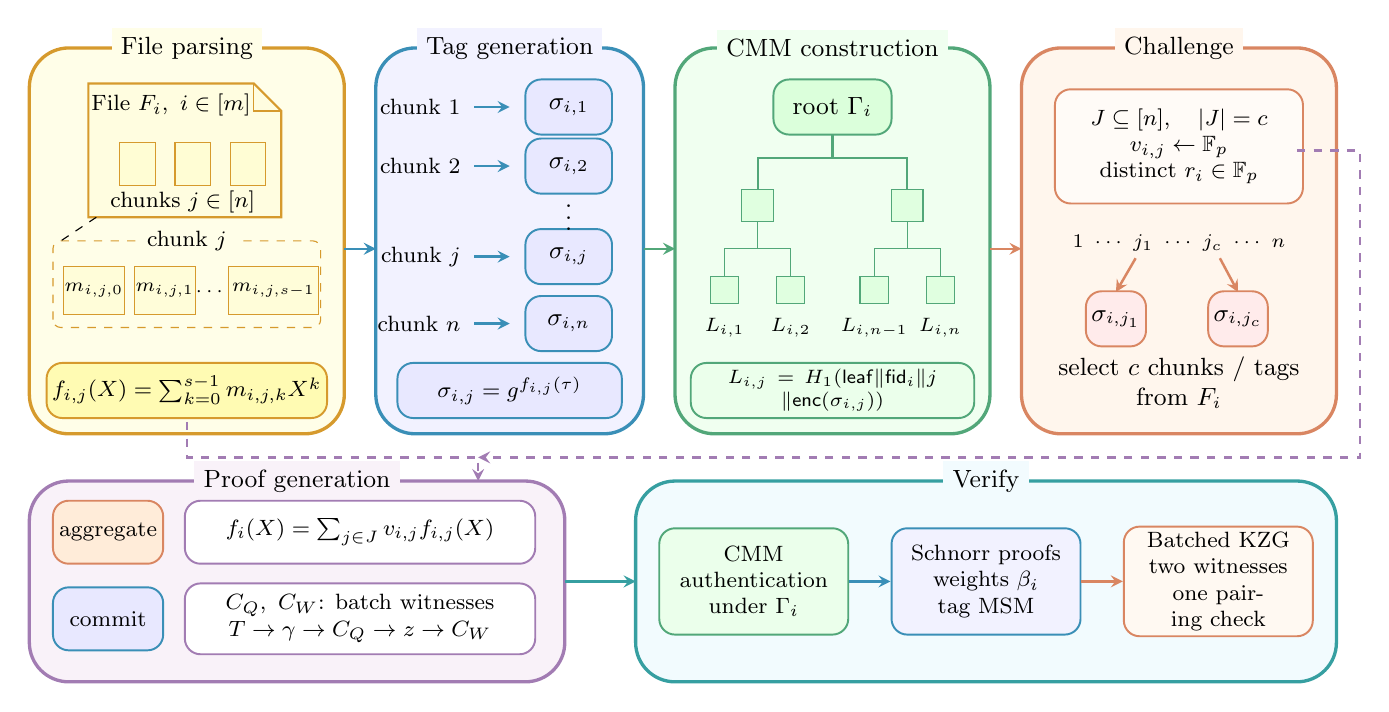
\begin{tikzpicture}[x=1cm,y=1cm,>=stealth,
 every node/.style={font=\small,align=center},
 panel/.style={rounded corners=5mm,line width=1.2pt},
 box/.style={rounded corners=2mm,line width=0.7pt,minimum height=7mm,inner sep=2pt},
 arrow/.style={->,line width=0.9pt}]
\definecolor{flowGold}{HTML}{D69A2D}
\definecolor{flowBlue}{HTML}{3A8FB7}
\definecolor{flowGreen}{HTML}{52A779}
\definecolor{flowOrange}{HTML}{D98662}
\definecolor{flowPurple}{HTML}{A27CB3}
\definecolor{flowTeal}{HTML}{369FA1}
% File parsing, tagging, per-file authentication, and challenge.
\draw[panel,draw=flowGold,fill=yellow!9] (0,2.7) rectangle (4,7.6);
\draw[panel,draw=flowBlue,fill=blue!5] (4.4,2.7) rectangle (7.8,7.6);
\draw[panel,draw=flowGreen,fill=green!6] (8.2,2.7) rectangle (12.2,7.6);
\draw[panel,draw=flowOrange,fill=orange!7] (12.6,2.7) rectangle (16.6,7.6);
\node[fill=yellow!9] at (2,7.6) {File parsing};
\node[fill=blue!5] at (6.1,7.6) {Tag generation};
\node[fill=green!6] at (10.2,7.6) {CMM construction};
\node[fill=orange!7] at (14.6,7.6) {Challenge};
\draw[draw=flowGold,line width=0.8pt,fill=yellow!12]
 (0.75,5.45)--(3.2,5.45)--(3.2,6.8)--(2.85,7.15)--(0.75,7.15)--cycle;
\draw[draw=flowGold] (2.85,7.15)--(2.85,6.8)--(3.2,6.8);
\node[font=\footnotesize] at (1.8,6.87) {File $F_i,\ i\in[m]$};
\foreach \x in {1.15,1.85,2.55}
 {\draw[draw=flowGold,fill=yellow!17] (\x,5.85) rectangle +(0.45,0.55);}
\node[font=\footnotesize] at (1.95,5.65) {chunks $j\in[n]$};
\draw[dashed,draw=flowGold,rounded corners=1mm] (0.3,4.05) rectangle (3.7,5.15);
\node[fill=yellow!9,font=\footnotesize] at (2,5.15) {chunk $j$};
\foreach \x/\lab/\halfw in {0.82/0/0.39,1.72/1/0.39,3.1/{s-1}/0.57}
 {\draw[draw=flowGold,fill=yellow!15] (\x-\halfw,4.22) rectangle (\x+\halfw,4.82);
  \node[font=\scriptsize] at (\x,4.52) {$m_{i,j,\lab}$};}
\node[font=\scriptsize] at (2.31,4.5) {$\cdots$};
\draw[dashed] (0.85,5.45)--(0.4,5.15);
\node[box,draw=flowGold,fill=white!70!yellow,minimum width=3.5cm,font=\footnotesize]
 at (2,3.25) {$f_{i,j}(X)=\sum_{k=0}^{s-1}m_{i,j,k}X^k$};
\foreach \yy/\jj in {6.85/1,6.1/2,4.95/j,4.1/n}
 {\node[anchor=east,font=\footnotesize] at (5.6,\yy) {chunk $\jj$};
  \draw[arrow,flowBlue] (5.65,\yy)--(6.1,\yy);
  \node[box,draw=flowBlue,fill=blue!9,minimum width=1.1cm] at (6.85,\yy) {$\sigma_{i,\jj}$};}
\node at (6.85,5.55) {$\vdots$};
\node[box,draw=flowBlue,fill=blue!9,minimum width=2.85cm,font=\footnotesize]
 at (6.1,3.25) {$\sigma_{i,j}=g^{f_{i,j}(\tau)}$};
\node[box,draw=flowGreen,fill=green!14,minimum width=1.5cm] at (10.2,6.85) {root $\Gamma_i$};
\draw[draw=flowGreen,line width=0.8pt] (10.2,6.5)--(10.2,6.2)--(9.25,6.2)--(9.25,5.8);
\draw[draw=flowGreen,line width=0.8pt] (10.2,6.2)--(11.15,6.2)--(11.15,5.8);
\foreach \xx in {9.25,11.15}
 {\draw[draw=flowGreen,fill=green!12] (\xx-0.2,5.4) rectangle (\xx+0.2,5.8);
  \draw[draw=flowGreen] (\xx,5.4)--(\xx,5.05)--(\xx-0.42,5.05)--(\xx-0.42,4.7);
  \draw[draw=flowGreen] (\xx,5.05)--(\xx+0.42,5.05)--(\xx+0.42,4.7);}
\foreach \xx/\jj in {8.83/1,9.67/2,10.73/{n-1},11.57/n}
 {\draw[draw=flowGreen,fill=green!12] (\xx-0.18,4.35) rectangle (\xx+0.18,4.7);
  \node[font=\scriptsize] at (\xx,4.05) {$L_{i,\jj}$};}
\node[box,draw=flowGreen,fill=green!8,text width=3.35cm,minimum width=3.6cm,font=\scriptsize]
 at (10.2,3.25) {$L_{i,j}=H_1(\mathsf{leaf}\|\mathsf{fid}_i\|j$\\$\|\mathsf{enc}(\sigma_{i,j}))$};
\node[box,draw=flowOrange,fill=orange!3,minimum width=3.15cm,minimum height=1.45cm,font=\footnotesize]
 at (14.6,6.35) {$J\subseteq[n],\quad |J|=c$\\$v_{i,j}\leftarrow\FF_p$\\distinct $r_i\in\FF_p$};
\node[text width=3.45cm,font=\scriptsize] at (14.6,5.12) {$1\ \cdots\ j_1\ \cdots\ j_c\ \cdots\ n$};
\draw[arrow,flowOrange] (14.05,4.93)--(13.8,4.5);
\draw[arrow,flowOrange] (15.12,4.93)--(15.35,4.5);
\node[box,draw=flowOrange,fill=red!8] at (13.8,4.16) {$\sigma_{i,j_1}$};
\node[box,draw=flowOrange,fill=red!8] at (15.35,4.16) {$\sigma_{i,j_c}$};
\node at (14.6,3.35) {select $c$ chunks / tags\\from $F_i$};
\draw[arrow,flowBlue] (4,5.05)--(4.4,5.05);
\draw[arrow,flowGreen] (7.8,5.05)--(8.2,5.05);
\draw[arrow,flowOrange] (12.2,5.05)--(12.6,5.05);
% Proof generation and verification.
\draw[panel,draw=flowPurple,fill=violet!5] (0,-0.45) rectangle (6.8,2.1);
\draw[panel,draw=flowTeal,fill=cyan!5] (7.7,-0.45) rectangle (16.6,2.1);
\node[fill=violet!5] at (3.4,2.1) {Proof generation};
\node[fill=cyan!5] at (12.15,2.1) {Verify};
\node[box,draw=flowOrange,fill=orange!15,minimum width=1.4cm,minimum height=8mm,font=\footnotesize] at (1,1.45) {aggregate};
\node[box,draw=flowPurple,fill=white,minimum width=4.45cm,minimum height=8mm,font=\footnotesize]
 at (4.2,1.45) {$f_i(X)=\sum_{j\in J}v_{i,j}f_{i,j}(X)$};
\node[box,draw=flowBlue,fill=blue!9,minimum width=1.4cm,minimum height=8mm,font=\footnotesize] at (1,0.35) {commit};
\node[box,draw=flowPurple,fill=white,minimum width=4.45cm,minimum height=9mm,font=\footnotesize]
 at (4.2,0.35) {$C_Q,\ C_W$: batch witnesses\\$T\to\gamma\to C_Q\to z\to C_W$};
\node[box,draw=flowGreen,fill=green!8,text width=2.1cm,minimum width=2.4cm,minimum height=1.35cm,font=\footnotesize]
 (tagAuth) at (9.2,0.825) {CMM\\authentication\\under $\Gamma_i$};
\node[box,draw=flowBlue,fill=blue!5,text width=2.1cm,minimum width=2.4cm,minimum height=1.35cm,font=\footnotesize]
 (maskCheck) at (12.15,0.825) {Schnorr proofs\\weights $\beta_i$\\tag MSM};
\node[box,draw=flowOrange,fill=orange!5,text width=2.1cm,minimum width=2.4cm,minimum height=1.35cm,font=\footnotesize]
 (openingCheck) at (15.1,0.825) {Batched KZG\\two witnesses\\one pairing check};
\draw[arrow,flowTeal] (6.8,0.825)--(7.7,0.825);
\draw[arrow,flowBlue] (tagAuth.east)--(maskCheck.west);
\draw[arrow,flowOrange] (maskCheck.east)--(openingCheck.west);
\draw[arrow,flowPurple,dashed] (2,2.85)--(2,2.4)--(5.7,2.4)--(5.7,2.1);
\draw[arrow,flowPurple,dashed] (16.1,6.3)--(16.9,6.3)--(16.9,2.4)--(5.7,2.4);
\end{tikzpicture}%
}
\caption{System model and audit workflow of MultiAudit. Sampled tags are authenticated by per-file CMMs; masked data openings are verified with two batch-opening witnesses.}
\label{fig:system model flowchar}
\end{figure*}

\paragraph{\textbf{Setup}}
The $\Setup$ algorithm initializes the cryptographic environment and publishes the system-wide public parameters $\mathsf{pp}$. It first generates a bilinear group tuple $(\GG_1, \GG_2, \GG_T, e)$ of prime order $p$, selects public generators $g \in \GG_1$ and $h \in \GG_2$, and samples a secret trapdoor $\tau \in \FF_p$. Using $\tau$, the algorithm constructs the structured reference string \(\SRS=(g,g^{\tau}, \dots, g^{\tau^{s-1}}, h, h^{\tau})\), which supports polynomial commitments of degree strictly less than $s$. Cryptographic hash functions are fixed: $H_1$ for Merkle tree construction, and $H_2$ for Fiat--Shamir transcript binding. Finally, $\mathsf{pp} = (\GG_1, \GG_2, \GG_T, e, p, g, h, \SRS, H_1, H_2)$ is published. Each DO initializes an independent trapdoor and SRS for its own file set; the trapdoor is not disclosed to the CS or V, while the published SRS is used for proof generation and verification. Only files sharing this SRS are batched together. Setup publishes a unique SRS identifier and protocol/version domains for base transcripts, $\gamma$, $z$, and Schnorr challenges. Hash-to-field uses rejection sampling of uniform $\lceil\log_2p\rceil$-bit strings until the integer lies below $p$, followed by rejection of zero for $\gamma$ or any $r_i$ for $z$. A domain-separated counter supplies fresh hash blocks, giving unbiased accepted samples in the random oracle model.
\begin{algorithm}[h]
\caption{$\Setup$}
\begin{algorithmic}[1]
\Require security parameter $\lambda$
\Ensure public parameters $\mathsf{pp}$
\State Generate $(\GG_1,\GG_2,\GG_T,e,p,g,h)$ and $\SRS=\left(g,g^\tau,\ldots,g^{\tau^{s-1}},h,h^\tau\right)$.
\State Fix $H_1,H_2$, canonical encodings, SRS identifier, and distinct transcript domains; use unbiased hash-to-field sampling.
\State Publish
$
\mathsf{pp}=(\GG_1,\GG_2,\GG_T,e,p,g,h,\SRS, H_1,H_2).
$
\end{algorithmic}
\end{algorithm}

\paragraph{\textbf{File Storage}}
The $\Store$ algorithm handles data preprocessing, cryptographic tagging, and metadata generation for outsourcing. For each file $F_i$ ($i \in [m]$), the Data Owner parses every chunk $j \in [n]$ into $s$ field elements and algebraically encodes them as a polynomial $f_{i,j}(X) = \sum_{k=0}^{s-1} m_{i,j,k} X^k$. A KZG homomorphic tag $\sigma_{i,j} = g^{f_{i,j}(\tau)} \in \GG_1$ is computed for each chunk, providing a compact cryptographic binding to the underlying data sectors. Since \(\tau\) is known to the DO, the tag is computed by evaluating \(f_{i,j}(\tau)\) over \(\FF_p\) and then performing one base exponentiation in \(\GG_1\).
Then, each tag is encoded as a domain-separated Merkle leaf $L_{i,j}=H_1(\mathsf{leaf}\|\mathsf{fid}_i\|j\|\mathsf{enc}(\sigma_{i,j}))$, and the leaves are organized into a Merkle tree with root $\Gamma_i$. The CMM primitive in Section~\ref{subsec:multiproofs} is instantiated independently for each file with $\mathsf{id}=\mathsf{fid}_i$, $X_j=\sigma_{i,j}$, and $\Gamma=\Gamma_i$; its auxiliary hash list and count are denoted by $\mathcal A_i(J)$ and $|\mathcal A_i(J)|$. The tree uses that primitive's public shape and domain-separated padding. The tree roots $\{\Gamma_i\}$ are securely retained by the DO (and later shared with the Verifier), while the raw data and tags are outsourced to the CS.

\begin{algorithm}[h]
\caption{$\Store$}
\label{alg:store}
\begin{algorithmic}[1]
\Require files $\{F_i\}_{i=1}^m$
\Ensure outsourced data, metadata
\For{$i=1$ to $m$}
  \For{$j=1$ to $n$}
    \State Parse chunk $j$ into $s$ sectors and form $f_{i,j}(X)$.
    \State Compute tag $\sigma_{i,j}=g^{f_{i,j}(\tau)}$.
    \State $L_{i,j}\gets H_1(\mathsf{leaf}\|\mathsf{fid}_i\|j\|\mathsf{enc}(\sigma_{i,j}))$.
  \EndFor
  \State Build the $i$th Merkle tree over leaves $\{L_{i,j}\}_{j=1}^n$.
  \State Obtain root $\Gamma_i$.
\EndFor
\State DO sends $(F_i,\{\sigma_{i,j}\})$ to CS and records $\{\Gamma_i\}$ for V.
\end{algorithmic}
\end{algorithm}

\paragraph{\textbf{Challenge Generation}}
The $\Chal$ algorithm initiates the audit by sampling a challenge tuple $\mathsf{chal} = (J, \{v_{i,j}\}_{i\in[m],j\in J}, \{r_i\}_{i=1}^m,\mathsf{nonce})$. An index set $J \subseteq [n]$ of size $c$ is selected and applied to every audited file. Independent coefficients $\{v_{i,j}\}$ are drawn uniformly from $\FF_p$ to randomize each file's linear aggregation. Distinct file-specific evaluation points $\{r_i\}$ are sampled uniformly without replacement from $\FF_p$ to support the batched opening check, while a fresh $\mathsf{nonce}$ prevents replay and precomputation attacks.

\begin{algorithm}[h]
\caption{$\Chal$}
\label{alg:chal}
\begin{algorithmic}[1]
\Require parameters $(m,n,c)$ with $1\leq c\leq n$, $1\leq m<p$, $s\geq2$
\Ensure challenge $\mathsf{chal}$
\State Sample $J\subseteq[n]$ uniformly without replacement, $|J|=c$.
\State Sample random $\{v_{i,j} \xleftarrow{\$}\FF_p\}_{i\in[m],j\in J}$.
\State Sample ordered distinct $(r_1,\ldots,r_m)$ uniformly without replacement from $\FF_p$.
\State Sample a fresh $\mathsf{nonce}$
\State Set
$
\mathsf{chal}=(J,\{v_{i,j}\}_{i\in[m],j\in J}, \{r_i\}_{i=1}^m, \mathsf{nonce}).
$
\end{algorithmic}
\end{algorithm}

\paragraph{Transcript and challenge order.}
Let $\mathcal M=((\mathsf{fid}_i,\mathsf{version}_i,n,s,\Gamma_i))_{i=1}^m$ be the current ordered, authenticated registry. Positions in the batch are not persistent file identifiers. Define the length-framed base transcript
\begin{equation}\label{eq:base_transcript}
\begin{split}
T=\mathsf{enc}(\mathcal M,\mathsf{chal},((\sigma_{i,j})_{j\in J},\tilde y_i,R_i)_{i=1}^m).
\end{split}
\end{equation}
All sequences follow registry order, with increasing $J$. Hash challenges are
\begin{equation}\label{eq:batch_challenges}
\begin{aligned}
\gamma&=H_{2,\gamma}(T)\in\FF_p^*,\\
z&=H_{2,z}(T,C_Q)\in\FF_p\setminus\{r_1,\ldots,r_m\},\\
\chi_i&=H_{2,\mathsf{mask}}((T,C_Q,C_W,i),R_i,A_i)\in\FF_p.
\end{aligned}
\end{equation}
The three domains are independent. CMM auxiliary hashes are checked against the bound roots; the authenticated tag values themselves are in $T$. The prover must fix $C_Q$ before learning $z$.

\paragraph{\textbf{Proof Generation}}
For each file the CS aggregates challenged chunks in the field, evaluates at $r_i$, and samples fresh masks. For honest masked claims, $P_i=f_i+\mu_i$ satisfies $P_i(X)-\tilde y_i=f_i(X)-f_i(r_i)$, so polynomial division in Section~\ref{subsec:polynomial_basics} gives the same quotient $q_i(X)$ as for the unmasked evaluation. The CS aggregates quotient coefficients and makes the following two SRS commitments:
\begin{equation}\label{eq:two_witnesses}
\begin{aligned}
q_i(X)&=\frac{f_i(X)-f_i(r_i)}{X-r_i},\quad
\beta_i=\frac{\gamma^{i-1}}{z-r_i},\\
C_Q&=g^{\sum_{i=1}^m\gamma^{i-1}q_i(\tau)},
\quad C_W=g^{\sum_{i=1}^m\beta_iq_i(\tau)}.
\end{aligned}
\end{equation}
Both witnesses commit to coefficient-wise sums over the common SRS. The Schnorr primitive in Section~\ref{subsec:schnorr} uses $Y=R_i$, $x=\mu_i$, $\mathsf d=\mathsf{mask}$, and $\mathsf{ctx}=(T,C_Q,C_W,i)$. Its nonce, commitment, challenge, and response $(t,A,\chi,\zeta)$ are written $(t_i,A_i,\chi_i,z_i)$, respectively.

\begin{algorithm}[t]
\caption{\textbf{$\ProofGen$}}
\label{alg:proofgen}
\begin{algorithmic}[1]
\Require $\mathsf{chal}$, ordered registry $\mathcal M$, files, tags, Merkle trees, common $\mathsf{pp}$
\Ensure proof $\pi$
\For{$i=1$ to $m$}
\State Collect $(\sigma_{i,j})_{j\in J}$ and generate the CMM auxiliary hash list $\mathcal A_i(J)$.
\State $f_i(X)\gets\sum_{j\in J}v_{i,j}f_{i,j}(X)$; $y_i\gets f_i(r_i)$.
\State Sample $\mu_i\leftarrow\FF_p$; $\tilde y_i\gets y_i+\mu_i$; $R_i\gets g^{\mu_i}$.
\State $q_i(X)\gets(f_i(X)-y_i)/(X-r_i)$.
\EndFor
\State Encode $T$ by Equation~\eqref{eq:base_transcript}; derive $\gamma$ by Equation~\eqref{eq:batch_challenges}.
\State Aggregate $Q=\sum_i\gamma^{i-1}q_i$ in the field; $C_Q\gets g^{Q(\tau)}$.
\State Derive $z$ by Equation~\eqref{eq:batch_challenges}; set $\beta_i=\gamma^{i-1}/(z-r_i)$.
\State Aggregate $W=\sum_i\beta_iq_i$ in the field; $C_W\gets g^{W(\tau)}$.
\For{$i=1$ to $m$}
\State Sample $t_i\leftarrow\FF_p$; $A_i\gets g^{t_i}$.
\State Derive $\chi_i$ by Equation~\eqref{eq:batch_challenges}; $z_i\gets t_i+\chi_i\mu_i$.
\EndFor
\State \Return $\pi=\bigl(((\sigma_{i,j})_{j\in J},\mathcal A_i,\tilde y_i,R_i,A_i,z_i)_{i=1}^m,C_Q,C_W\bigr)$.
\end{algorithmic}
\end{algorithm}

\paragraph{\textbf{Verification}}
The verifier first validates the current registry, the challenge, group/subgroup membership, and canonical encodings. It authenticates all sampled tags using one CMM per file and checks each Schnorr equation. Authenticated tags determine $b_i=\prod_{j\in J}\sigma_{i,j}^{v_{i,j}}$, a verifier-local quantity. The batch-opening statement in Section~\ref{subsec:batch_openings} is instantiated by $B_i=b_iR_i$ and $u_i=\tilde y_i$. It checks
\begin{equation}\label{eq:batch_pairing}
\begin{aligned}
D&=C_Q^{-1}\prod_{i=1}^m(b_iR_i g^{-\tilde y_i})^{\beta_i},\\
e(DC_W^z,h)&\stackrel{?}{=}e(C_W,h^\tau).
\end{aligned}
\end{equation}
Implementation evaluates the left group argument as one MSM as described in Section~\ref{sec:complexity_analysis}; constructing the intermediate $b_i$ is unnecessary.

\begin{algorithm}[t]
\caption{\textbf{$\Verify$}}
\label{alg:verify}
\begin{algorithmic}[1]
\Require $\mathsf{chal}$, proof $\pi$, current authenticated registry $\mathcal M$, common $\mathsf{pp}$
\Ensure $\mathsf{accept}$ or $\mathsf{reject}$
\State Parse the exact proof format of Algorithm~\ref{alg:proofgen}; reject invalid lengths, encodings, or subgroup elements.
\State Reject unless the registry is current, all SRS identifiers agree, $J$ is sorted with $|J|=c$, and all $r_i$ are distinct.
\For{$i=1$ to $m$}
\State Reconstruct $\Gamma_i$ from $(\sigma_{i,j})_{j\in J}$ and $\mathcal A_i$ by the canonical traversal; reject on failure or unused hashes.
\EndFor
\State Encode $T$ by Equation~\eqref{eq:base_transcript}; derive $\gamma,z$ by Equation~\eqref{eq:batch_challenges}.
\For{$i=1$ to $m$}
\State Derive $\chi_i$ by Equation~\eqref{eq:batch_challenges}.
\If{$g^{z_i}\ne A_iR_i^{\chi_i}$}
\State \Return $\mathsf{reject}$.
\EndIf
\State Set $\beta_i=\gamma^{i-1}/(z-r_i)$ and $b_i=\prod_{j\in J}\sigma_{i,j}^{v_{i,j}}$ (conceptually).
\EndFor
\State Form $D$ and check Equation~\eqref{eq:batch_pairing}; reject if it fails.
\State \Return $\mathsf{accept}$.
\end{algorithmic}
\end{algorithm}
The mask proofs establish knowledge of $\mu_i$, not knowledge of the data coefficients. Authentication and data-opening verification share $T$; failed batch verification does not identify a faulty file.

\subsection{Security Analysis}
We analyze the construction. All adversaries are PPT in $\lambda$; all roots and the ordered active-file registry are authenticated. The owner-generated tags fix the underlying chunk polynomials, and the server does not know the SRS trapdoor.

\begin{theorem}[Correctness]\label{thm:correctness}
Honest executions of Algorithms~\ref{alg:store}--\ref{alg:verify} accept for every valid challenge and accepted hash-to-field output.
\end{theorem}
\begin{proof}
CMMs reconstruct the registered roots. Homomorphism gives $b_i=g^{f_i(\tau)}$, and Schnorr correctness gives $g^{z_i}=A_iR_i^{\chi_i}$. Let $P_i=f_i+\mu_i$, so $g^{P_i(\tau)}=b_iR_i$ and $P_i(r_i)=\tilde y_i$. Using Equation~\eqref{eq:two_witnesses},
\begin{equation}\label{eq:batch_identity}
\begin{split}
&\sum_i\beta_i(P_i(X)-\tilde y_i)-Q(X)\\
&=\sum_i\bigl(\beta_i(X-r_i)-\gamma^{i-1}\bigr)q_i(X)\\
&=(X-z)\sum_i\beta_iq_i(X)=(X-z)W(X).
\end{split}
\end{equation}
The middle equality uses $\beta_i(z-r_i)=\gamma^{i-1}$. At $X=\tau$, this gives $D=g^{(\tau-z)W(\tau)}$, hence $DC_W^z=g^{\tau W(\tau)}$ and Equation~\eqref{eq:batch_pairing} follows by bilinearity.
\end{proof}

\begin{theorem}[Soundness]\label{thm:soundness}
Assume Assumptions~\ref{ass:hash},~\ref{ass:batch_opening_agm},~\ref{ass:random_oracle}, and~\ref{ass:schnorr_knowledge}. For extracted masks $\mu_i$, let $P_i=f_i+\mu_i$ be determined by the authenticated tags. If some $P_i(r_i)\ne\tilde y_i$, then, for one fresh second-challenge query with statements and $C_Q$ already fixed, acceptance has probability at most
\[
\frac{m+s-1}{p-m}+\varepsilon_{\rm red},
\]
where $\varepsilon_{\rm red}$ includes $\varepsilon_{\rm alg}(\lambda)$ from Assumption~\ref{ass:batch_opening_agm}, together with authentication and Schnorr extraction failures. Over at most $Q_z$ fresh second-challenge inputs and one unqueried final input,
\begin{equation}\label{eq:batch_query_bound}
\begin{split}
&\Pr[\mathsf{accept}\land\mathsf{false\ claim}]\\
&\quad\leq\min\left\{1,\frac{(Q_z+1)(m+s-1)}{p-m}
+\varepsilon_{\rm red}\right\}.
\end{split}
\end{equation}
The reduction error is for the whole execution, including its oracle queries; it is not asserted to follow from evaluation binding alone.
\end{theorem}
\begin{proof}
Condition on successful authentication and extraction. For analysis, $P_i$ and the extracted degree-$<s$ polynomial $Q$ are fixed before the response to a fresh $z$ query. Define the rational function
\[
\mathcal R(Z)=\sum_i\gamma^{i-1}\frac{P_i(Z)-\tilde y_i}{Z-r_i}-Q(Z).
\]
If claim $k$ is false, the pole at $r_k$ has nonzero residue $\gamma^{k-1}(P_k(r_k)-\tilde y_k)$. Other terms have no pole there because the $r_i$ are distinct; $Q$ is a polynomial and $\gamma\ne0$. Thus $\mathcal R$ is not the zero rational function. Multiplying by $V(Z)=\prod_i(Z-r_i)$ yields a nonzero polynomial of degree at most $m+s-1$, where this conservative bound allows a malicious $Q$ to use the full SRS degree. By Lemma~\ref{lem:schwartz_zippel}, it has at most $m+s-1$ roots among the $p-m$ allowed values of $z$.
Under Assumption~\ref{ass:batch_opening_agm} with $u_i=\tilde y_i$, an accepting pairing implies $G_z(z)=\mathcal R(z)=0$, except on the reduction failure event. Rejection sampling makes each fresh accepted $z$ uniform on the allowed set. Applying the conditional root bound before each fresh query and a union bound proves Equation~\eqref{eq:batch_query_bound}. An already queried input supplies no new random draw. Grinding over different $T$, $\gamma$, or $C_Q$ is covered by the number of fresh $z$ inputs. Without fixing $C_Q$ first, the prover could choose $Q$ after seeing $z$ to force $\mathcal R(z)=0$, invalidating the bound.
\end{proof}

\begin{samepage}
\begin{theorem}[Public Verifiability]\label{thm:public_verifiability}
Under the assumptions of Theorem~\ref{thm:soundness}, MultiAudit satisfies public verifiability as specified in Section~\ref{sec:security_model}.
\end{theorem}
\begin{proof}
Algorithm~\ref{alg:verify} uses only $\mathsf{pp},\mathcal M,\mathsf{chal},\pi$: CMM reconstruction, transcript challenges, Schnorr checks, MSMs, and pairings are public deterministic computations. It never evaluates a polynomial at the secret $\tau$. Theorems~\ref{thm:correctness} and~\ref{thm:soundness} give honest acceptance and the stated false-opening bound for any party using the same authenticated inputs.
\end{proof}
\end{samepage}

\begin{proposition}[Evaluation-Masking Privacy]\label{prop:leakage}
MultiAudit satisfies evaluation-masking privacy as specified in Section~\ref{sec:security_model}. Nevertheless, every honest public transcript reveals $U_i=g^{\tilde y_i}R_i^{-1}=g^{f_i(r_i)}$, permitting candidate-evaluation tests. Full-transcript evaluation indistinguishability is therefore not provided.
\end{proposition}

\begin{proof}
For every $\mathbf a,\mathbf b\in\FF_p^m$, fresh independent uniform masks give $\Pr[\tilde{\mathbf y}=\mathbf a\mid\mathbf y=\mathbf b]=\Pr[\boldsymbol\mu=\mathbf a-\mathbf b]=p^{-m}$. The argument also holds conditional on prior audits because masks are refreshed. However, $\tilde y_i=y_i+\mu_i$ and $R_i=g^{\mu_i}$ imply $U_i=g^{y_i}$. Any candidate $y'$ is tested by $g^{y'}=U_i$; distinct field evaluations give distinct encodings. Marginal scalar privacy therefore does not extend to the complete verifier view.
\end{proof}

\subsection{Complexity Analysis}
\label{sec:complexity_analysis}
We count scalar terms in $\GG_1$ ($\CompExp$), scalar terms in $\GG_2$ ($\CompExp'$), and pairing terms ($\CompPair$). These are algebraic term counts before MSM acceleration, not independent-operation latency estimates. A public-SRS commitment counts one scalar term per coefficient; a tag generated with the DO-known trapdoor costs one $\CompExp$. Hash-to-group calls implemented as base scalar multiplications also count as $\CompExp$. Field operations, byte hashing, and serialization must be measured separately. Let $L=\lceil\log_2n\rceil$ and $A_\Sigma(J)=\sum_{i=1}^m |\mathcal A_i(J)|$ be the total number of auxiliary hashes transmitted across the independent file trees.

\paragraph{Computation.}
Storage uses $mn\CompExp$ for tags, $\mathcal O(mns)$ field operations for their trapdoor evaluations, and $\mathcal O(mn)$ hashes for independent trees. Public-SRS-only storage without a retained trapdoor would have a different tag-generation cost and is outside this Store convention.

Proof generation aggregates $m$ challenged polynomials, evaluates them, and computes their quotients in $\mathcal O(mcs)$ field operations. Each of $Q$ and $W$ has at most $s-1$ coefficients and is committed \emph{after} coefficient aggregation, costing $2(s-1)\CompExp$ in total. The $m$ mask commitments and $m$ Schnorr commitments cost $2m\CompExp$. Thus
\begin{equation}\label{eq:proofgen_cost}
\mathsf{Cost}_{\ProofGen}=[2(s-1)+2m]\CompExp.
\end{equation}
Coefficient aggregation for both witnesses adds $\mathcal O(ms)$ field operations. The $\beta_i$ use $m$ inverses, or one inversion and $\mathcal O(m)$ multiplications with batch inversion. These inversions and hash-to-field rejection sampling are outside the scalar-term count. CMM generation gathers $A_\Sigma(J)$ hashes from stored trees and traverses the sampled branches; it does not regenerate all nodes.

For verification, expand $b_i$ directly into the pairing's left argument:
\begin{equation}\label{eq:verify_msm}
\begin{split}
L_{\rm data}=DC_W^z
= {}& C_Q^{-1}C_W^z\,
g^{-\sum_i\beta_i\tilde y_i}\cdot\prod_i R_i^{\beta_i}
\prod_i\prod_{j\in J}\sigma_{i,j}^{\beta_i v_{i,j}}.
\end{split}
\end{equation}
This MSM has $mc+m+2$ scalar terms: $mc$ tags, $m$ masks, one generator, and $C_W$; $C_Q^{-1}$ is a group inversion, not a scalar multiplication. Independent Schnorr checks add $2m\CompExp$, and the final equation uses two pairings with the fixed $h,h^\tau$ (no $\GG_2$ scalar multiplication). Hence
\begin{equation}\label{eq:verify_cost}
\mathsf{Cost}_{\Verify}=(mc+3m+2)\CompExp+2\CompPair.
\end{equation}
Auxiliary hash lists and sampled tag encodings incur hash and parsing costs; for per-file trees root reconstruction uses $m$ times the leaf/internal-node hash count specified after Equation~\eqref{eq:aux_count} when all tree shapes agree. These costs are measured separately from Equation~\eqref{eq:verify_cost}.

\paragraph{Communication.}
Using bit lengths $|p|$, $|\GG_1|$, and $|h|$ for a scalar, group element, and hash, respectively, one-time outsourcing is unchanged:
\[
mns|p|+mn|\GG_1|+m|h|.
\]
The response contains $mc$ sampled tags, $m$ mask commitments, $m$ Schnorr commitments, two witnesses, and $2m$ scalars (masked values and Schnorr responses). Its payload is
\begin{equation}\label{eq:response_cost}
(mc+2m+2)|\GG_1|+2m|p|+A_\Sigma(J)|h|.
\end{equation}
The response includes all sampled tags. Challenges, identifiers, setup keys, and wire framing are excluded from this payload convention.

\subsection{Dynamic File Management}
Dynamic support is a central requirement in practical PDP systems~\cite{Erway2009DPDP,Wang2011TPDS,Yang2013TPDS,XuTIFS26}. In many outsourced-storage services, files are added and deleted much more frequently than audit rounds are executed: a user may update the active dataset continuously, while the auditor checks integrity hourly, daily, or according to a compliance schedule. MultiAudit supports file addition and active audit-set removal through independent per-file KZG commitments and modular Merkle trees; chunk-level updates are outside this scope. Crucially, $\ProofGen$ and $\Verify$ are stateless per audit round; they operate on the current active file set without maintaining persistent or incremental proof state. Dynamic operations thus only affect the $\Store$ phase and metadata synchronization.

When the DO uploads a new file $F_{m+1}$, it encodes each chunk into $f_{m+1,j}(X)$, computes tags $\sigma_{m+1,j}=g^{f_{m+1,j}(\tau)}$, and constructs a fresh Merkle tree yielding root $\Gamma_{m+1}$. The data and tags are outsourced to the CS, while $\Gamma_{m+1}$ is securely shared with the verifier. The number of active files increments to $m \leftarrow m+1$. No existing file tag, Merkle root, quotient witness, or global accumulator is recomputed. At the next scheduled audit, $F_{m+1}$ is automatically incorporated through the expanded active file identifier set and Merkle root set.

To remove $F_{i_{\text{del}}}$ from subsequent audits, the DO and V revoke $\Gamma_{i_{\text{del}}}$ from the active metadata set and exclude the corresponding file identifier from future challenges. The CS may reclaim the associated data, tags, and Merkle nodes according to the storage policy, but this protocol action is only an audit-set update and does not prove physical erasure. Surviving files simply skip the removed identifier in subsequent audit loops, incurring zero recomputation of tags or Merkle roots. The number of active files decreases by one, and future $\ProofGen$ executions simply iterate over the reduced active set.

\textit{Complexity of Dynamic Operations.} Adding a single file requires $\mathcal{O}(n\CompExp)$ time for tag generation, as implied by the \textsf{Store} algorithm under the DO-known trapdoor computation. Removing a file from the active audit set only updates the metadata registry and requires no tag generation, Merkle reconstruction for surviving files, SRS regeneration, trapdoor rotation, or global commitment recomputation. Since proof generation is challenge-driven and stateless, dynamic updates incur overhead strictly at the storage and metadata layers. Consequently, the \textsf{ProofGen} and \textsf{Verify} algorithms retain the same complexity as analyzed in Section~\ref{sec:complexity_analysis}.

\section{Related Works}
\label{sec:related_works}

\begin{table*}[!t]
\centering
\caption{Computational Complexity Comparison (Scalar Terms $\CompExp,\CompExp'$ Before MSM and Pairings $\CompPair$) in Multi-File Setting}
\label{tab:computation}
\renewcommand{\arraystretch}{1.3}
\begin{tabular}{l|c|c|c}
\hline
\textbf{Scheme} & \textbf{$\Store$} & \textbf{$\ProofGen$} & \textbf{$\Verify$} \\
\hline
Xu et al.~\cite{XuTIFS26} (TIFS26) & $mn\CompExp$ & $m(s-1)\CompExp+\mathcal{O}(mcs\CompField)$ & $(mc+1)\CompExp+\CompExp'+2\CompPair$ \\
Zhang et al.~\cite{ZhangTPDS23} (TPDS23) & $3mn\CompExp$& $(mc+2s-2)\CompExp+\mathcal{O}((mcs+m^2s)\CompField)$& $(2mc+2)\CompExp+\CompExp'+4\CompPair$\\
Yu et al.~\cite{YuTC25} (TC25) & $mn\CompExp$ & $m\CompExp+\mathcal{O}(mcs\CompField)$ & $m(c+2s+1)\CompExp$\\
Miao et al.~\cite{MiaoSCIS2026} (SCIS26) &  $(m\ell+2m+3mn_{\mathrm M})\CompExp$ & $(mc+1)\CompExp+\mathcal{O}(mc\CompField)$ & $(2mc+m+2)\CompExp+2\CompPair$\\
\hline
\textbf{MultiAudit} & $mn\CompExp$ & $[2(s-1)+2m]\CompExp+\mathcal{O}(mcs\CompField)$ & $(mc+3m+2)\CompExp+2\CompPair$ \\
\hline
\end{tabular}
\footnotesize
\begin{minipage}{0.96\textwidth}
\(\CompField\) appears only in \textsf{ProofGen} and denotes one modular addition or multiplication over \(\FF_p\) in polynomial aggregation, evaluation, and quotient computation; it excludes inversion, exponentiation, hashing, scalar decoding, and group operations. The \(mcs\)-scaled terms mainly affect Yu et al.~\cite{YuTC25}, Xu et al.~\cite{XuTIFS26}, and MultiAudit; Zhang et al.~\cite{ZhangTPDS23} leverage PCS for multiple points and polynomials (PCS-MPAP)~\cite{Boneh2020PCS}, whereas Miao et al.~\cite{MiaoSCIS2026} have only \(\mathcal{O}(mc\CompField)\).
\end{minipage}
\end{table*}

\begin{table*}[!t]
\centering
\caption{Communication Complexity Comparison (in bits) in Multi-File Setting}
\label{tab:communication}
\renewcommand{\arraystretch}{1.3}
\begin{tabular}{l|c|c}
\hline
\textbf{Scheme} & \textbf{$\Store$ Phase} & \textbf{$\ProofGen$ Phase} \\
\hline
Xu et al.~\cite{XuTIFS26} (TIFS26) & $mns|p|+mn|\GG_1|+m|h|$& $m\bigl(|p|+(c+1)|\GG_1|+c\lceil\log_2 n\rceil|h|\bigr)$\\
Zhang et al.~\cite{ZhangTPDS23} (TPDS23) & $mns|p| + mn|\GG_1|$& $3|\GG_1| + |p|$\\
Yu et al.~\cite{YuTC25} (TC25) & $mns|p| + mn|\GG_1| + m|h|$& $m\big(s|p| + (c+1)|\GG_1| + c\lceil\log_2 n\rceil|h|\big)$\\
Miao et al.~\cite{MiaoSCIS2026} (SCIS26) & $mn_{\mathrm M}|p|+(mn_{\mathrm M}+m)|\GG_1|$ & $|p|+2|\GG_1|$ \\
\hline
\textbf{MultiAudit} & $mns|p|+mn|\GG_1|+m|h|$ & $(mc+2m+2)|\GG_1|+2m|p|+A_\Sigma(J)|h|$ \\
\hline
\end{tabular}
\end{table*}

The PDP model of Ateniese et al.~\cite{Ateniese2007PDP} checks outsourced data through probabilistic challenges and homomorphic authenticators. Juels and Kaliski~\cite{Juels2007POR}, and subsequently Shacham and Waters~\cite{Shacham2008POR}, develop proofs of retrievability, which additionally address recovery through extraction. We review authentication mechanisms, update support, audit scope, and proof-generation efficiency as complementary design dimensions; a construction can contribute to several of them.

\paragraph{Merkle-Based Tag Authentication}
Merkle trees bind tags to positions under an authenticated root, complementing the algebraic tag relation. Liu et al.~\cite{Liu2015MuRDPA} use a multi-replica Merkle structure, and Rao et al.~\cite{Rao2020BatchMHT} develop batch-leaf authentication for dynamic outsourced auditing. Xu et al.~\cite{XuTIFS26} combine Merkle authentication with polynomial commitments; Yu et al.~\cite{YuTC25} use a tag-indexed Merkle hash tree (Tag-IMHT). Hash-based authentication provides explicit index and membership checks, but independent paths duplicate sibling hashes when challenged branches overlap. The CMMs of Ramabaja and Avdullahu~\cite{Ramabaja2020Compact} merge these paths without changing the authenticated values. MultiAudit applies one CMM to each file's sampled tags. This reduces authentication traffic while preserving independent roots, although the response still carries the sampled tags and a challenge-dependent number of auxiliary hashes.

\paragraph{Polynomial and Vector Commitment Tags}
KZG~\cite{Kate2010KZG} provides constant-size polynomial commitments and evaluation witnesses. Vector commitments introduced by Catalano and Fiore~\cite{Catalano2013VC} authenticate indexed values, while Campanelli et al.~\cite{Campanelli20ASIACRYPT} provide incrementally aggregatable subvector openings in hidden-order groups. Accumulator batching is studied by Boneh et al.~\cite{Boneh2019Batching}. These primitives offer different setup, update, and witness-generation trade-offs and should be distinguished from complete auditing protocols. In storage auditing, Du et al.~\cite{Du22TDSC} use polynomial commitments for blockchain-assisted decentralized verification; Yu et al.~\cite{Yu2024Edasvic} combine polynomial-commitment authenticators with an authenticator accumulator. Yu et al.~\cite{Yu2024EDCOMA} further investigate double-compressed auditing for decentralized storage. Such approaches reduce selected proof or metadata components, but compact commitments alone do not make an entire audit response constant-size. MultiAudit uses KZG for data tags and two-witness batch openings~\cite[Sec.~4.1]{Boneh2020PCS} for their evaluation claims; CMMs separately authenticate the tags entering those claims.

\paragraph{PDP with Dynamic Updates}
Update support requires maintaining both authenticators and current indexing information. Ateniese et al.~\cite{Ateniese2008Scalable} study efficient symmetric-key PDP with restricted updates, whereas Erway et al.~\cite{Erway2009DPDP} develop dynamic PDP using authenticated structures. Wang et al.~\cite{Wang2011TPDS} and Yang and Jia~\cite{Yang2013TPDS} combine public auditing with data dynamics. Shen et al.~\cite{Shen2017Dynamic} design a specialized dynamic structure, while Duan et al.~\cite{Duan2023DecentralizedAudit} reduce the auditor-state and proof costs of dynamic decentralized storage. Barsoum and Hasan~\cite{Barsoum2015Multicopy} address multicopy dynamics, and Zhou et al.~\cite{Zhou2022Certificateless} support certificateless multicopy auditing with batch updates. These capabilities require update protocols and metadata synchronization beyond a static audit equation. MultiAudit's narrower scope is file addition and removal from the active audit set: independent roots avoid rebuilding surviving files. It does not provide chunk-level insertion, deletion, modification, or proof of physical erasure.

\paragraph{Multi-File and Multi-Replica Auditing}
Curtmola et al.~\cite{Curtmola2008MRPDP} study possession of multiple replicas; this requirement differs from batching independently managed files. Xu et al.~\cite{XuTIFS26} support aggregation across files and providers in multi-copy storage, using a shared evaluation point. Zhang et al.~\cite{ZhangTPDS23} use PCS-MPAP at distinct file-specific points and obtain a constant-size per-provider response, retaining a communication advantage over protocols that transmit sampled tags. Miao et al.~\cite{MiaoSCIS2026} aggregate proofs over keyword-matched files and authenticate search-result completeness, addressing a selection requirement absent from ordinary batch auditing. In contrast, Yu et al.~\cite{YuTC25} provide a single-file construction; multiple files require separate executions. MultiAudit batches authenticated opening claims at distinct points under a common SRS while maintaining independent file roots. Its theorem concerns false evaluation claims for the authenticated tags, rather than replica uniqueness or general data retrievability. Shared evaluation points alone do not establish insecurity in other constructions.

\paragraph{Proof-Generation Efficiency}
Reducing response size, prover computation, and verifier computation are distinct objectives. Xu et al.~\cite{XuTIFS26} compute a quotient commitment per file, giving the $m(s-1)\CompExp$ proof-generation term in Table~\ref{tab:computation}. MultiAudit aggregates quotient coefficients before committing, replacing this term with two aggregate commitments and per-file mask proofs, for $[2(s-1)+2m]\CompExp$. This reduces group scalar terms while retaining $\mathcal O(mcs\CompField)$ challenged-data aggregation; it therefore does not imply a proportional runtime improvement. Yu et al.~\cite{YuTC25} avoid pairing verification and return quotient coefficients, obtaining inexpensive proof generation at the cost of a larger scalar component. Zhang et al.~\cite{ZhangTPDS23} and Miao et al.~\cite{MiaoSCIS2026} retain constant-size responses with different tag-processing and verification costs.

Efficiency also depends on deployment and trust assumptions. Shu et al.~\cite{Shu2022BlockchainAudit} decentralize public auditing with blockchain, and Liu et al.~\cite{Liu2025TLARDA} study threshold label aggregation. Chen et al.~\cite{Chen2024ObjectAuditing} examine practical object-storage auditing, while Chen et al.~\cite{Chen2024ServerlessAuditing} supply auditing computation through serverless infrastructure. These system-level approaches complement algebraic proof compression. Privacy is a separate comparison dimension: Wang et al.~\cite{Wang2013TC} study privacy-preserving public auditing, and Oruta~\cite{Wang2014TCC} protects signer identity in shared-data auditing. MultiAudit proves marginal evaluation masking but exposes public evaluation encodings that permit candidate testing. Consequently, its computational and communication benefits do not establish full-transcript confidentiality or subsume the broader functionality of the comparison protocols.

Tables~\ref{tab:computation} and~\ref{tab:communication} compare analytically derived group-operation and communication costs. We set $L=\lceil\log_2n\rceil$. MultiAudit uses independent per-file Merkle trees. The Store column counts group work; Merkle hashing is accounted for separately in Section~\ref{sec:complexity_analysis}. Yu's privacy-enhanced variant executes $m$ independent audits; Xu and Zhang are normalized to one replica/provider. Miao uses $n_{\mathrm M}=ns$ single-scalar blocks for equal encoded file bytes, and $\ell$ is its average keyword count per file. Sampling the same number of native blocks therefore does not imply equal coverage.

The computation metric omits group additions/inversions, byte hashing, field inversion/exponentiation, scalar conversion, PRFs, and searchable-index processing. Dominant proof-generation field additions/multiplications are included separately as $\CompField$; the two witnesses add coefficient aggregation and weight derivation as detailed in Section~\ref{sec:complexity_analysis}. The payload convention excludes challenges, identifiers, setup keys, searchable-index metadata, and wire framing. Independent paths have $L$ hashes; CMM sizes use actual auxiliary counts, not $cL$.

\paragraph{Illustrative encoding-normalized comparison.}
For $(m,s,c,n)=(40,80,690,3907)$, assume 48-byte $\GG_1$ elements and 32-byte scalars and hashes. These are uniform encoding assumptions; Section~\ref{sec:evaluation} uses the backend's actual 64-byte group encodings. For a uniformly sampled $c$-subset of $[n]$ and a subtree $B$ containing $k_B$ real positions,
\[
\Pr[B\text{ touched}]=1-\frac{\binom{n-k_B}{c}}{\binom nc}.
\]
Summing these probabilities over internal subtrees and subtracting $c-1$, by the reconstruction count after Equation~\eqref{eq:aux_count}, gives $\mathbb E[|\mathcal A_i(J)|]\simeq1332.89$ and $\mathbb E[A_\Sigma(J)]\simeq53315.62$. Actual response sizes depend on $J$.

MultiAudit reduces server scalar terms from $3160E$ to $238E$ relative to Xu et al.~\cite{XuTIFS26}, a 92.5\% reduction. The corresponding expected response reduction under this illustrative encoding is 74.5\%. Both protocols retain $\mathcal O(mcs)$ field aggregation; measured latency also includes authentication, allocation and transcript work. Zhang et al.~\cite{ZhangTPDS23} and Miao et al.~\cite{MiaoSCIS2026} retain constant-response advantages.

% BEGIN GENERATED EVALUATION
\section{Evaluation}
\label{sec:evaluation}
\subsection{Experimental Setup}
We fix nominal 10~MB files (10,001,920 encoded bytes), $s=80$, $c=690$, and $n=3907$ for the multi-sector layout, with 64-byte $\GG_1$ elements and 32-byte scalars/hashes. Baseline normalization follows Tables~\ref{tab:computation} and~\ref{tab:communication}.

PC tests use Go~1.25.4 (\texttt{darwin/arm64}) on an Apple M4 (10 logical cores, 16~GiB RAM, macOS~26.5.2). All schemes share BN256 (go-ethereum~v1.17.2), Pippenger MSM, and field/storage kernels. We vary $m\in\{10,20,30,40\}$; Miao et al.~\cite{MiaoSCIS2026} uses two keywords per file and queries all files. All configurations use complete stored fixtures. Online calls use one worker and a locked OS thread; 30 fresh audits follow at least three warmups and five seconds of warmup. We report medians/interquartile ranges without sample removal. Store is measured once (up to four file workers for the searchable scheme, sequential otherwise). Setup, synthetic-input and challenge generation, response encoding, and transfer are excluded. GC is requested outside online timers; collections during calls remain included.

The single-file chain experiment uses Ganache~7.9.2 (Shanghai), Solidity~0.8.25 with optimization/via-IR, and a 100~Mgas local block limit. Five fresh audits per scheme share BN254/SHA-256 helpers and EIP-1108~\cite{EIP1108} prices. Bilinearity moves Xu's $\GG_2$ scalar multiplication to $\GG_1$; Yu combines $(X-z)q(X)+y$ before its SRS MSM; MultiAudit uses Equation~\eqref{eq:verify_msm}. A different account submits ABI proofs against owner-registered roots/SRS and challenge digests; indices occupy 32 bytes. Receipt gas includes calldata and execution; deployment and prior registration are excluded.

The Release SwiftUI client runs on a physical iPhone~13 (iOS~26.6.2; Xcode~26.1), using the shared Go code as an ARM64 library. For $m=10$, the phone performs fresh owner setup and sequential Store; the host runs ProofGen with public parameters. Local Verify is optional and enabled in these tests. Store sums native per-file preprocessing, excluding setup, input construction, encoding, and network waiting. Upload bytes include files and signed-registry bodies (fixed-width root slots), excluding HTTP/TCP headers. Thirty fresh audits follow three warmups. Core Verify excludes decoding; client Verify includes decoding and the common Swift/Go interface. Both exclude network waiting.

\subsection{Sampling Coverage and Parameter Selection}
\label{subsec:sampling_coverage}
The following calculation motivates the common challenge size.

\begin{lemma}[Sampling Coverage]\label{lem:overall_acceptance}
Fix a target file with $n$ chunks and a corruption set of actual size $d$ fixed before sampling. If $c\leq n$ indices are sampled uniformly without replacement, then
\begin{equation}
P_{\mathrm{miss}}=\frac{\binom{n-d}{c}}{\binom nc},
\qquad P_{\mathrm{hit}}=1-P_{\mathrm{miss}},
\end{equation}
where $0\leq d\leq n$, $1\leq c$, and $\binom{n-d}{c}=0$ when $c>n-d$.
\end{lemma}

\begin{proof}
Of the $\binom nc$ equally likely challenge sets, exactly $\binom{n-d}{c}$ avoid the fixed corruption set. The hit probability is the complement.
\end{proof}

For $\delta=d/n$, $P_{\mathrm{miss}}\approx(1-\delta)^c$ when the finite-population correction is small, e.g., $c^2/(n-d)\ll1$ with $n-d>0$. If $A$ denotes final acceptance and $M$ a sampling miss, total probability gives
\begin{equation}
\begin{split}
\Pr[A]=P_{\mathrm{miss}}\Pr[A\mid M]+(1-P_{\mathrm{miss}})\Pr[A\mid M^c].
\end{split}
\end{equation}
Zero-weight conditional terms are omitted. A sampling hit need not imply a false opening claim, so Theorem~\ref{thm:soundness} does not bound $\Pr[A\mid M^c]$ without an additional data-possession argument.

\begin{remark}[Sampling Parameter Selection]\label{rem:parameter_selection}
For a fixed corruption fraction $\delta=d/n$, $P_{\mathrm{miss}}\leq(1-\delta)^c$; thus $c\geq\ln\epsilon/\ln(1-\delta)$ suffices for sampling-hit probability $1-\epsilon$, provided $c\leq n$. At approximately $1\%$ corruption, $c\approx690$ gives about $99.9\%$ sampling-hit probability in the large-population approximation. The exact probability uses the actual count $d$ in Lemma~\ref{lem:overall_acceptance}. This is sampling coverage, not a protocol detection rate.
\end{remark}

\subsection{PC Results}
\label{subsec:pc_results}
\begin{figure*}[!t]
\centering

\begin{tikzpicture}[font=\sffamily\footnotesize]
\begin{scope}[xshift=0pt]
\filldraw[fill=XuTIFS26!75,draw=XuTIFS26!90!black,line width=0.35pt] (0pt,-3pt) rectangle (10pt,4pt);
\node[anchor=west,inner sep=0pt] at (16pt,0pt) {Xu et al.~\cite{XuTIFS26}};
\end{scope}
\begin{scope}[xshift=100pt]
\filldraw[fill=ZhangTPDS23!75,draw=ZhangTPDS23!90!black,line width=0.35pt] (0pt,-3pt) rectangle (10pt,4pt);
\node[anchor=west,inner sep=0pt] at (16pt,0pt) {Zhang et al.~\cite{ZhangTPDS23}};
\end{scope}
\begin{scope}[xshift=200pt]
\filldraw[fill=YuTC25!75,draw=YuTC25!90!black,line width=0.35pt] (0pt,-3pt) rectangle (10pt,4pt);
\node[anchor=west,inner sep=0pt] at (16pt,0pt) {Yu et al.~\cite{YuTC25}};
\end{scope}
\begin{scope}[xshift=300pt]
\filldraw[fill=MiaoSCIS2026!75,draw=MiaoSCIS2026!90!black,line width=0.35pt] (0pt,-3pt) rectangle (10pt,4pt);
\node[anchor=west,inner sep=0pt] at (16pt,0pt) {Miao et al.~\cite{MiaoSCIS2026}};
\end{scope}
\begin{scope}[xshift=400pt]
\filldraw[fill=MultiAudit,draw=MultiAudit!90!black,line width=0.35pt] (0pt,-3pt) rectangle (10pt,4pt);
\node[anchor=west,inner sep=0pt] at (16pt,0pt) {MultiAudit};
\end{scope}
\end{tikzpicture}
\par\smallskip
\subfloat[Store (s)]{\begin{minipage}{0.33\textwidth}\centering
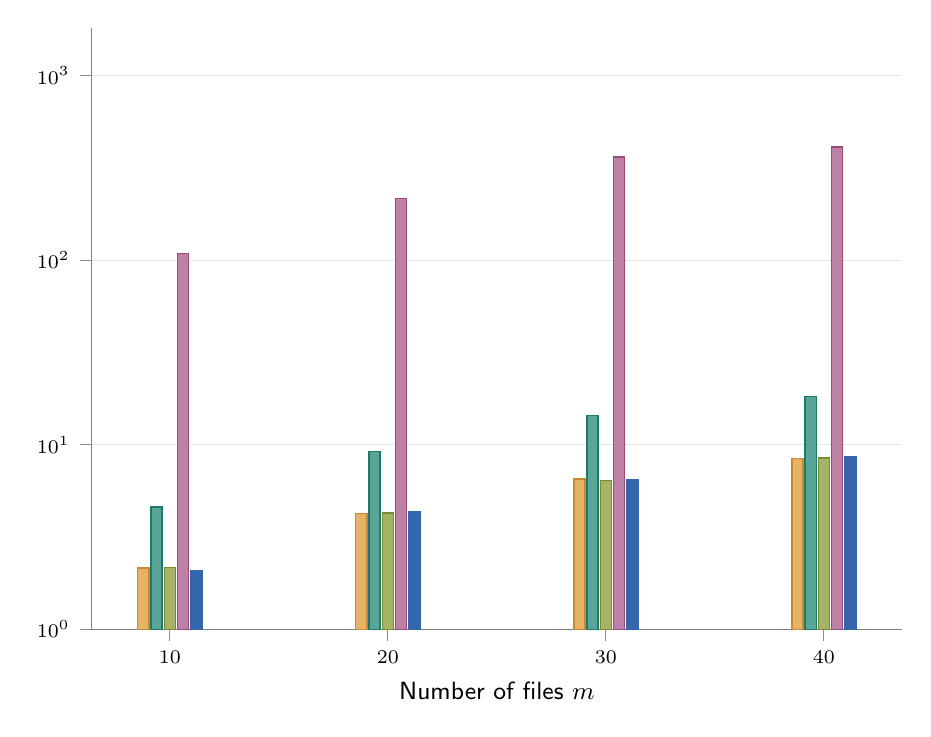
\begin{tikzpicture}
\begin{axis}[auditaxis,xlabel={Number of files $m$},ylabel={},xtick={10,20,30,40},ybar=0.8pt,bar width=4pt,ymode=log,log origin=infty,ymin=1.00000000,ymax=677.403855]
\addplot+[draw=XuTIFS26!90!black,fill=XuTIFS26!75,line width=0.5pt] coordinates {(10,2.14583646) (20,4.25551975) (30,6.53334788) (40,8.41894892)};
\addplot+[draw=ZhangTPDS23!90!black,fill=ZhangTPDS23!75,line width=0.5pt] coordinates {(10,4.60361938) (20,9.18189200) (30,14.36089033) (40,18.26398604)};
\addplot+[draw=YuTC25!90!black,fill=YuTC25!75,line width=0.5pt] coordinates {(10,2.16836821) (20,4.26029242) (30,6.40219808) (40,8.45803717)};
\addplot+[draw=MiaoSCIS2026!90!black,fill=MiaoSCIS2026!75,line width=0.5pt] coordinates {(10,108.16028800) (20,215.21035700) (30,361.68253287) (40,410.54779100)};
\addplot+[draw=MultiAudit,fill=MultiAudit,line width=0.6pt] coordinates {(10,2.07794833) (20,4.33284121) (30,6.49087742) (40,8.56814862)};
\end{axis}
\end{tikzpicture}

\end{minipage}}
\hfill
\subfloat[ProofGen (ms)]{\begin{minipage}{0.33\textwidth}\centering
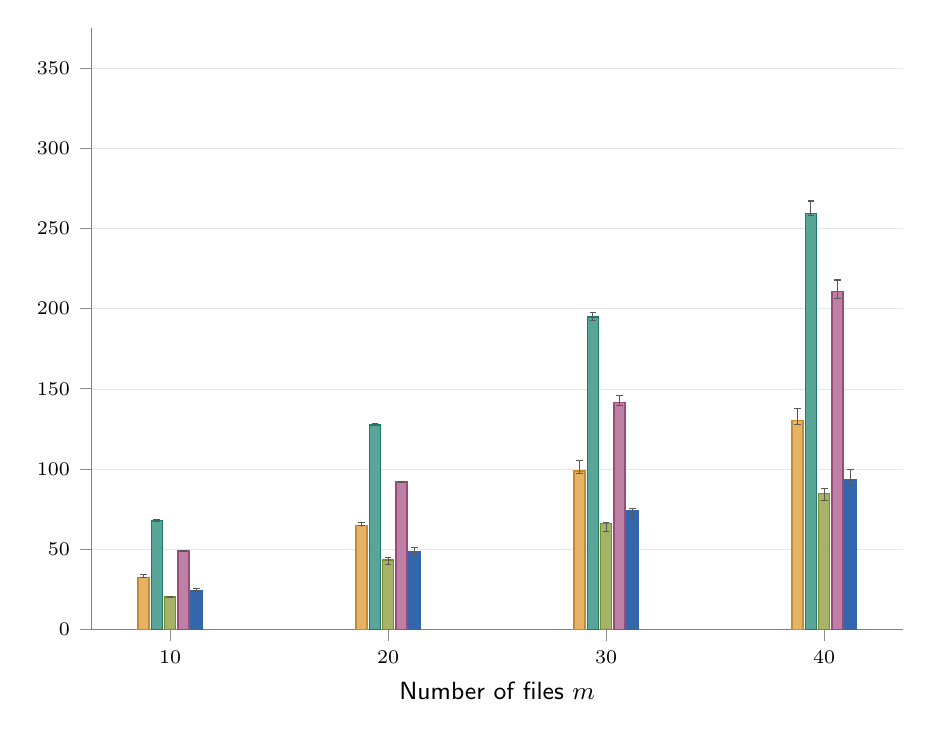
\begin{tikzpicture}
\begin{axis}[auditaxis,xlabel={Number of files $m$},ylabel={},xtick={10,20,30,40},ybar=0.8pt,bar width=4pt,ymin=0,ymax=325.966132]
\addplot+[draw=XuTIFS26!90!black,fill=XuTIFS26!75,line width=0.5pt,error bars/.cd,y dir=both,y explicit,error bar style={color=black!65,draw=black!65,line width=0.4pt},error mark options={draw=black!65,rotate=90,mark size=1.2pt,line width=0.4pt}] coordinates {(10,32.37979100) += (0,1.90179200) -= (0,0.09548900) (20,64.74275000) += (0,1.83062500) -= (0,0.16235400) (30,98.74508400) += (0,6.67821800) -= (0,1.30927200) (40,130.24791700) += (0,7.48319800) -= (0,2.52007300)};
\addplot+[draw=ZhangTPDS23!90!black,fill=ZhangTPDS23!75,line width=0.5pt,error bars/.cd,y dir=both,y explicit,error bar style={color=black!65,draw=black!65,line width=0.4pt},error mark options={draw=black!65,rotate=90,mark size=1.2pt,line width=0.4pt}] coordinates {(10,67.83739600) += (0,0.90735400) -= (0,0.39121800) (20,127.33912500) += (0,0.81155200) -= (0,0.28804100) (30,194.75635300) += (0,2.78864700) -= (0,2.02685300) (40,259.19937500) += (0,7.98597900) -= (0,0.96921800)};
\addplot+[draw=YuTC25!90!black,fill=YuTC25!75,line width=0.5pt,error bars/.cd,y dir=both,y explicit,error bar style={color=black!65,draw=black!65,line width=0.4pt},error mark options={draw=black!65,rotate=90,mark size=1.2pt,line width=0.4pt}] coordinates {(10,20.12008300) += (0,0.12694800) -= (0,0.19907300) (20,43.34270800) += (0,1.27906300) -= (0,2.62100000) (30,65.85302100) += (0,0.89722900) -= (0,4.56533300) (40,84.57877100) += (0,3.05555100) -= (0,4.40220800)};
\addplot+[draw=MiaoSCIS2026!90!black,fill=MiaoSCIS2026!75,line width=0.5pt,error bars/.cd,y dir=both,y explicit,error bar style={color=black!65,draw=black!65,line width=0.4pt},error mark options={draw=black!65,rotate=90,mark size=1.2pt,line width=0.4pt}] coordinates {(10,48.76410500) += (0,0.34952000) -= (0,0.45748000) (20,91.83677100) += (0,0.55796800) -= (0,0.36559300) (30,141.41850000) += (0,4.39425000) -= (0,1.84041700) (40,210.57016700) += (0,7.30085400) -= (0,4.44023000)};
\addplot+[draw=MultiAudit,fill=MultiAudit,line width=0.6pt,error bars/.cd,y dir=both,y explicit,error bar style={color=black!65,draw=black!65,line width=0.4pt},error mark options={draw=black!65,rotate=90,mark size=1.2pt,line width=0.4pt}] coordinates {(10,24.15987500) += (0,1.15786400) -= (0,0.22864600) (20,48.34400000) += (0,2.76686400) -= (0,1.70995800) (30,73.67745900) += (0,1.81934400) -= (0,5.02828200) (40,93.15787500) += (0,6.80807200) -= (0,3.50086500)};
\end{axis}
\end{tikzpicture}

\end{minipage}}
\hfill
\subfloat[Verify (ms)]{\begin{minipage}{0.33\textwidth}\centering
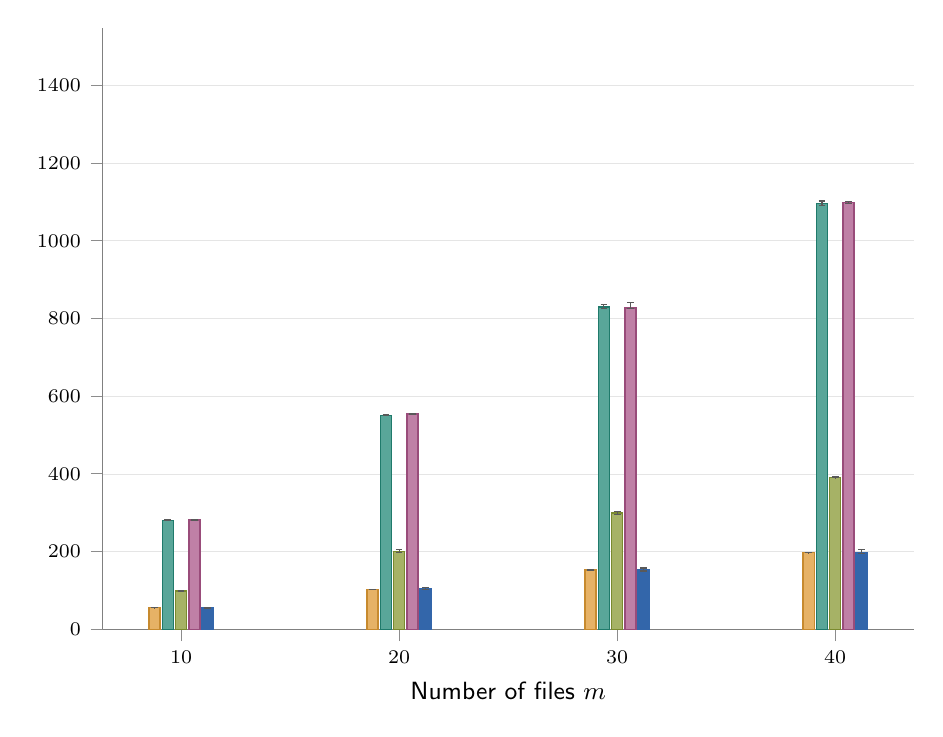
\begin{tikzpicture}
\begin{axis}[auditaxis,xlabel={Number of files $m$},ylabel={},xtick={10,20,30,40},ybar=0.8pt,bar width=4pt,ymin=0,ymax=1345.140661]
\addplot+[draw=XuTIFS26!90!black,fill=XuTIFS26!75,line width=0.5pt,error bars/.cd,y dir=both,y explicit,error bar style={color=black!65,draw=black!65,line width=0.4pt},error mark options={draw=black!65,rotate=90,mark size=1.2pt,line width=0.4pt}] coordinates {(10,55.78764500) += (0,1.55913700) -= (0,0.14973900) (20,102.88820800) += (0,0.37909400) -= (0,0.27178100) (30,153.27456300) += (0,0.70948900) -= (0,1.39955200) (40,197.53277100) += (0,0.81822900) -= (0,0.30784400)};
\addplot+[draw=ZhangTPDS23!90!black,fill=ZhangTPDS23!75,line width=0.5pt,error bars/.cd,y dir=both,y explicit,error bar style={color=black!65,draw=black!65,line width=0.4pt},error mark options={draw=black!65,rotate=90,mark size=1.2pt,line width=0.4pt}] coordinates {(10,280.27412500) += (0,2.77393800) -= (0,0.80017700) (20,551.01849900) += (0,0.80594900) -= (0,0.63273900) (30,829.56779100) += (0,7.58999100) -= (0,4.14797800) (40,1095.28654200) += (0,7.28777000) -= (0,5.00094800)};
\addplot+[draw=YuTC25!90!black,fill=YuTC25!75,line width=0.5pt,error bars/.cd,y dir=both,y explicit,error bar style={color=black!65,draw=black!65,line width=0.4pt},error mark options={draw=black!65,rotate=90,mark size=1.2pt,line width=0.4pt}] coordinates {(10,98.36212400) += (0,0.24934500) -= (0,0.45816600) (20,200.22710400) += (0,4.53195800) -= (0,2.98575000) (30,299.74910400) += (0,3.48797900) -= (0,4.20417600) (40,390.58075000) += (0,3.23739600) -= (0,0.44839600)};
\addplot+[draw=MiaoSCIS2026!90!black,fill=MiaoSCIS2026!75,line width=0.5pt,error bars/.cd,y dir=both,y explicit,error bar style={color=black!65,draw=black!65,line width=0.4pt},error mark options={draw=black!65,rotate=90,mark size=1.2pt,line width=0.4pt}] coordinates {(10,281.49000000) += (0,1.82804200) -= (0,1.77345800) (20,553.79237500) += (0,1.65416700) -= (0,0.25584400) (30,827.19743700) += (0,13.28088600) -= (0,1.58021800) (40,1098.25637500) += (0,3.99499000) -= (0,1.48973900)};
\addplot+[draw=MultiAudit,fill=MultiAudit,line width=0.6pt,error bars/.cd,y dir=both,y explicit,error bar style={color=black!65,draw=black!65,line width=0.4pt},error mark options={draw=black!65,rotate=90,mark size=1.2pt,line width=0.4pt}] coordinates {(10,54.58218800) += (0,1.48481200) -= (0,0.22077100) (20,104.52106200) += (0,3.14677200) -= (0,2.27303100) (30,152.10297900) += (0,5.82650000) -= (0,1.77994700) (40,196.83843700) += (0,7.74367700) -= (0,0.66096800)};
\end{axis}
\end{tikzpicture}

\end{minipage}}
\caption{Runtime versus file count for $B=10$~MB per file, $s=80$, and $c=690$. Store is measured once in seconds on a logarithmic axis. Online bars show median milliseconds and interquartile ranges over 30 fresh audits.}
\label{fig:vi_runtime_sweeps}
\end{figure*}
\paragraph{Storage and scaling}
Fig.~\ref{fig:vi_runtime_sweeps}(a) shows approximately linear Store growth with file count. MultiAudit stays close to Xu et al.~\cite{XuTIFS26} and Yu et al.~\cite{YuTC25}, consistent with their common $mn\CompExp$ tag-generation term in Table~\ref{tab:computation}. Store still generates all chunk tags and complete per-file authentication trees. CMMs compact the sampled authentication paths during ProofGen, while coefficient aggregation reduces the opening-commitment work in that phase. Consequently, these improvements primarily benefit online auditing.

\paragraph{Proof generation}
Table~\ref{tab:computation} identifies the benefit of aggregating quotient coefficients before commitment: MultiAudit uses $[2(s-1)+2m]\CompExp$, replacing the $m(s-1)\CompExp$ witness term of Xu et al.~\cite{XuTIFS26}. Fig.~\ref{fig:vi_runtime_sweeps}(b) confirms lower proof-generation latency as the batch grows. At $m=40$, the speedups are 1.40$\times$ over Xu et al.~\cite{XuTIFS26} and 2.78$\times$ over Zhang et al.~\cite{ZhangTPDS23}. The latency gain is smaller than the scalar-term reduction because challenged-data aggregation remains $\mathcal O(mcs)$ and complete calls include field, authentication, and memory work. Yu et al.~\cite{YuTC25} retains faster ProofGen by returning quotient coefficients; Table~\ref{tab:communication} makes the corresponding response trade-off explicit.

\paragraph{Verification}
Fig.~\ref{fig:vi_runtime_sweeps}(c) is consistent with the verification terms in Table~\ref{tab:computation}: MultiAudit combines the openings into two pairing terms and one data MSM, while Yu et al.~\cite{YuTC25} repeats per-file checks and Zhang et al.~\cite{ZhangTPDS23} and Miao et al.~\cite{MiaoSCIS2026} have larger tag-related scalar terms. The verification speedup over Zhang et al.~\cite{ZhangTPDS23} reaches 5.56$\times$. The latency of Xu et al.~\cite{XuTIFS26} remains close to MultiAudit's: both retain the leading $mc$ tag term, while MultiAudit additionally checks masks and binds its transcript. Group counts explain the trends but are not proportional latency predictions under MSM acceleration.

\begin{figure}[t]
\centering
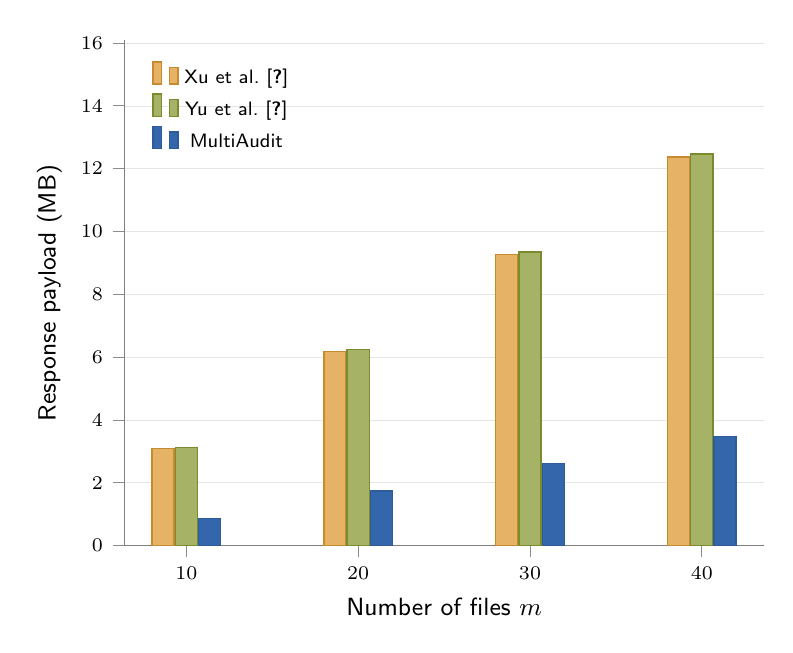
\begin{tikzpicture}
\begin{axis}[auditaxis,width=0.8\linewidth,height=0.66\linewidth,xlabel={Number of files $m$},ylabel={Response payload (MB)},xtick={10,20,30,40},ybar=0.4pt,bar width=8pt,ymin=0,ymax=14,legend style={font=\sffamily\scriptsize,draw=none,fill=none,at={(0.03,0.97)},anchor=north west,legend columns=1}]
\addplot+[draw=XuTIFS26!90!black,fill=XuTIFS26!75,line width=0.5pt] coordinates {(10,3.09216000) (20,6.18432000) (30,9.27648000) (40,12.36864000)};
\addlegendentry{Xu et al.~\cite{XuTIFS26}}
\addplot+[draw=YuTC25!90!black,fill=YuTC25!75,line width=0.5pt] coordinates {(10,3.11744000) (20,6.23488000) (30,9.35232000) (40,12.46976000)};
\addlegendentry{Yu et al.~\cite{YuTC25}}
\addplot+[draw=MultiAudit!90!black,fill=MultiAudit,line width=0.5pt] coordinates {(10,0.87017299) (20,1.74021797) (30,2.61026296) (40,3.48030794)};
\addlegendentry{MultiAudit}
\end{axis}
\end{tikzpicture}
\caption{Audit-response payload of Merkle-authenticated schemes at $B=10$~MB, $s=80$, and $c=690$. Native 64-byte groups and 32-byte scalars and hashes are used; MultiAudit uses expected CMM size. Framing is excluded. At $m=40$, MultiAudit reduces the expected payload by 71.9\% relative to Xu et al.~\cite{XuTIFS26}.}
\label{fig:vi_communication}
\end{figure}
\paragraph{Communication}
Table~\ref{tab:communication} explains the reduction in Fig.~\ref{fig:vi_communication}: CMMs replace the $mcL$ independent-path hashes with $A_\Sigma(J)$ auxiliary hashes, and the opening component uses two witnesses. The full response still includes sampled tags and per-file masks. At $m=40$, the mean encoded MultiAudit response is 71.9\% smaller than the native payload accounting of Xu et al.~\cite{XuTIFS26}. This comparison includes MultiAudit framing and excludes baseline framing; the plotted estimates exclude framing for every scheme and use expected CMM sizes. Zhang et al.~\cite{ZhangTPDS23} and Miao et al.~\cite{MiaoSCIS2026} retain constant-size cryptographic responses, so MultiAudit's communication advantage concerns the Merkle-authenticated baselines rather than every comparison scheme.

\subsection{On-Chain Costs}
\label{subsec:onchain_costs}
Table~\ref{tab:onchain_cost} shows that MultiAudit lowers both execution gas and calldata, reducing total gas by roughly one third relative to Xu et al.~\cite{XuTIFS26} and Yu et al.~\cite{YuTC25}. This agrees with Table~\ref{tab:communication}: CMMs avoid repeated authentication hashes, reducing both transmitted bytes and path reconstruction. Yu's pairing-free verifier still costs more overall, illustrating why the scalar/pairing counts in Table~\ref{tab:computation} must be read together with authentication and input costs. Since $m=1$, this experiment demonstrates a single-file benefit without exercising the witnesses' cross-file aggregation advantage. All 15 valid transactions succeed, and 21 tampered-input or unauthorized-update checks are rejected.

\begin{table}[t]
\centering
\caption{Measured Single-File EVM Verification ($s=80$, $B=10$~MB, $c=690$; Five Audits per Scheme)}
\label{tab:onchain_cost}
\small
\setlength{\tabcolsep}{3pt}
\begin{tabular*}{\columnwidth}{@{\extracolsep{\fill}}lrrr@{}}
\toprule
Scheme & \shortstack{Calldata\\(kB)} & \shortstack{Execution\\(Mgas)} & \shortstack{Total\\(Mgas)} \\
\midrule
Xu et al.~\cite{XuTIFS26} & 353.57 & 16.60 & 22.01 \\
Yu et al.~\cite{YuTC25} & 356.10 & 17.60 & 23.05 \\
\textbf{MultiAudit} & \textbf{130.56} & \textbf{12.69} & \textbf{14.54} \\
\bottomrule
\end{tabular*}
\par\smallskip
\footnotesize kB $=10^3$ bytes; Mgas $=10^6$ gas. Execution excludes transaction intrinsic gas; total includes it.
\end{table}
Applying the EIP-7623~\cite{EIP7623} calldata floor to the recorded inputs while holding measured execution fixed leaves these totals unchanged; this is a repricing projection, not a newer-fork measurement. Only MultiAudit's measured totals fit the $2^{24}$ transaction cap of EIP-7825~\cite{EIP7825}, so target-chain limits remain relevant even for a single file.

\subsection{iPhone Costs}
\label{subsec:iphone_costs}
Table~\ref{tab:mobile_costs} complements Tables~\ref{tab:computation} and~\ref{tab:communication}. For ten files, each scheme generates $mn=39{,}070$ tags and constructs complete per-file authentication trees during Store. The measured file uploads contain the same encoded sectors and tags, totaling 102,520,040 bytes per scheme; signed-registry bodies bring each application upload to approximately 102.54~MB. This common preprocessing explains the similar Store times. The cloud generates CMMs for the sampled set $J$ during ProofGen, reducing subsequent audit responses and authentication work. The two aggregate witnesses likewise target cloud ProofGen, leaving the initial tag and data upload unchanged.

MultiAudit reduces native Verify time by 5.4\% relative to Xu et al.~\cite{XuTIFS26} and 37.2\% relative to Yu et al.~\cite{YuTC25}. Including decoding and the shared language interface, complete local verification takes 157.53~ms, reductions of 23.6\% and 42.3\%, respectively. Relative to Xu, reduced authentication hashing helps despite comparable leading tag-MSM terms. Against Yu, batching also avoids repeated per-file opening checks. The larger client difference additionally reflects processing smaller audit responses.

\begin{table}[t]
\centering
\caption{Measured iPhone~13 Costs for Ten 10~MB Files ($s=80$, $c=690$)}
\label{tab:mobile_costs}
\small
\setlength{\tabcolsep}{2pt}
\begin{tabular*}{\columnwidth}{@{\extracolsep{\fill}}ccccc@{}}
\toprule
Scheme & \shortstack{Store\\(s)} & \shortstack{Store upload\\(MB)} & \shortstack{Core Verify\\(ms)} & \shortstack{Client Verify\\(ms)} \\
\midrule
Xu et al.~\cite{XuTIFS26} & 3.225 & 102.54 & 129.13 & 206.26 \\
Yu et al.~\cite{YuTC25} & 3.211 & 102.54 & 194.72 & 273.13 \\
\textbf{MultiAudit} & 3.243 & 102.54 & \textbf{122.22} & \textbf{157.53} \\
\bottomrule
\end{tabular*}
\par\smallskip
\footnotesize Store is one complete pass; Verify columns are medians of 30 audits. Core excludes decoding; client includes decoding and the common language interface. Uploads include signed-registry bodies; MB $=10^6$ bytes.
\end{table}

% END GENERATED EVALUATION

\section{Conclusion}

MultiAudit combines per-file CMMs with two-witness KZG openings under a common data SRS. Independent roots retain file addition and active audit-set removal. At $(m,B,s,c)=(40,10\,\mathrm{MB},80,690)$, the complete implementation takes 93.16~ms to generate a proof and 196.84~ms to verify it. The mean encoded response is 3474.65~kB, 71.9\% smaller than the native payload accounting of Xu et al.~\cite{XuTIFS26}. Group counts, measured latency and encoded response sizes are reported separately, with the shared optimized backends applied to every protocol. Constant-response and native-sampling trade-offs of the related constructions remain explicit. The physical iPhone~13 experiment additionally confirms comparable initial Store costs and lower optional verification costs than Xu et al.~\cite{XuTIFS26} and Yu et al.~\cite{YuTC25}, with ProofGen executed outside the phone.
\par
The security statement concerns authenticated opening claims under the stated algebraic and random-oracle assumptions. Verification is public given authenticated metadata; privacy is limited to marginal scalar masking. Neither general data possession, sector confidentiality, nor faulty-file localization is established. Honest transcripts still expose evaluation group encodings and permit candidate testing. At $m=1$, $B=10$~MB, and $s=80$, local-EVM verification consumes 14.54~Mgas, reducing median total gas by 33.9\% and 36.9\% relative to Xu et al.~\cite{XuTIFS26} and Yu et al.~\cite{YuTC25}; the measured fork and target-chain transaction limits remain explicit.

\IEEEtriggeratref{37}
\begin{thebibliography}{00}

\bibitem{ZhangTPDS23}
Q.~Zhang, Z.~Zhang, J.~Cui, H.~Zhong, Y.~Li, C.~Gu, and D.~He,
``Efficient blockchain-based data integrity auditing for multi-copy in decentralized storage,''
\emph{IEEE Trans. Parallel Distrib. Syst.}, vol.~34, no.~12, pp.~3162--3173, 2023.

\bibitem{XuTIFS26}
Y.~Xu, H.~Cheng, J.~Zheng, X.~Zhang, and H.~Wang,
``MPA: Lightweight and updatable integrity auditing for decentralized storage using Merkle trees and polynomial commitments,''
\emph{IEEE Trans. Inf. Forensics Security}, vol.~21, pp.~2162--2176, 2026.

\bibitem{YuTC25}
H.~Yu, H.~Zhang, Z.~Yang, Y.~Chen, and H.~Liu,
``Efficient and secure storage verification in cloud-assisted industrial IoT networks,''
\emph{IEEE Trans. Comput.}, vol.~74, no.~5, pp.~1702--1716, 2025.

\bibitem{Ateniese2007PDP}
G.~Ateniese, R.~Burns, R.~Curtmola, J.~Herring, L.~Kissner, Z.~Peterson, and D.~Song,
``Provable data possession at untrusted stores,''
in \emph{ACM CCS}, 2007, pp.~598--609.

\bibitem{Dinh2013MCC}
H.~T.~Dinh, C.~Lee, D.~Niyato, and P.~Wang,
``A survey of mobile cloud computing: Architecture, applications, and approaches,''
\emph{Wireless Commun. Mobile Comput.}, vol.~13, no.~18, pp.~1587--1611, 2013.

\bibitem{Li2015OPoR}
J.~Li, X.~Tan, X.~Chen, D.~S.~Wong, and F.~Xhafa,
``OPoR: Enabling proof of retrievability in cloud computing with resource-constrained devices,''
\emph{IEEE Trans. Cloud Comput.}, vol.~3, no.~2, pp.~195--205, 2015.

\bibitem{Yu2022Offline}
H.~Yu, Z.~Yang, S.~Tu, M.~Waqas, and H.~Liu,
``Blockchain-based offline auditing for the cloud in vehicular networks,''
\emph{IEEE Trans. Netw. Service Manag.}, vol.~19, no.~3, pp.~2944--2956, 2022.

\bibitem{Merkle1988}
R.~C.~Merkle,
``A digital signature based on a conventional encryption function,''
in \emph{CRYPTO 1987}, 1988, pp.~369--378.

\bibitem{Catalano2013VC}
D.~Catalano and D.~Fiore,
``Vector commitments and their applications,''
in \emph{PKC}, 2013, pp.~55--72.

\bibitem{Campanelli20ASIACRYPT}
M.~Campanelli, D.~Fiore, N.~Greco, D.~Kolonelos, and L.~Nizzardo,
``Incrementally aggregatable vector commitments and applications to verifiable decentralized storage,''
in \emph{ASIACRYPT}, 2020, pp.~3--35.

\bibitem{Kate2010KZG}
A.~Kate, G.~M.~Zaverucha, and I.~Goldberg,
``Constant-size commitments to polynomials and their applications,''
in \emph{ASIACRYPT}, 2010, pp.~177--194.

\bibitem{Ramabaja2020Compact}
L.~Ramabaja and A.~Avdullahu,
``Compact Merkle multiproofs,''
arXiv:2002.07648, 2020. [Online]. Available: \url{https://arxiv.org/abs/2002.07648}.

\bibitem{Boneh2020PCS}
D.~Boneh, J.~Drake, B.~Fisch, and A.~Gabizon,
``Efficient polynomial commitment schemes for multiple points and polynomials,''
Cryptology ePrint Archive, Paper 2020/081, 2020, revised May 2021. [Online]. Available: \url{https://eprint.iacr.org/2020/081}.

\bibitem{Schnorr1991Sig}
C.~P.~Schnorr,
``Efficient signature generation by smart cards,''
\emph{J. Cryptol.}, vol.~4, no.~3, pp.~161--174, 1991.

\bibitem{Wang2013TC}
C.~Wang, S.~S.~M.~Chow, Q.~Wang, K.~Ren, and W.~Lou,
``Privacy-preserving public auditing for secure cloud storage,''
\emph{IEEE Trans. Comput.}, vol.~62, no.~2, pp.~362--375, 2013.

\bibitem{MiaoSCIS2026}
Y.~Miao, K.~K.~Gai, and L.~Zhu,
``Blockchain-assisted multi-keyword searchable provable data possession for cloud storage,''
\emph{Sci. China Inf. Sci.}, vol.~69, no.~3, Art.~no.~132101, 2026.

\bibitem{Schwartz1980}
J.~T.~Schwartz,
``Fast probabilistic algorithms for verification of polynomial identities,''
\emph{J. ACM}, vol.~27, no.~4, pp.~701--717, 1980.

\bibitem{Fuchsbauer2018AGM}
G.~Fuchsbauer, E.~Kiltz, and J.~Loss,
``The algebraic group model and its applications,''
in \emph{CRYPTO}, Part~II, 2018, pp.~33--62.

\bibitem{FiatShamir1987}
A.~Fiat and A.~Shamir,
``How to prove yourself: Practical solutions to identification and signature problems,''
in \emph{CRYPTO 1986}, 1987, pp.~186--194.

\bibitem{BellareRogaway1993}
M.~Bellare and P.~Rogaway,
``Random oracles are practical: A paradigm for designing efficient protocols,''
in \emph{ACM CCS}, 1993, pp.~62--73.

\bibitem{Erway2009DPDP}
C.~Erway, A.~K{\"u}p{\c{c}}{\"u}, C.~Papamanthou, and R.~Tamassia,
``Dynamic provable data possession,''
in \emph{ACM CCS}, 2009, pp.~213--222.

\bibitem{Wang2011TPDS}
Q.~Wang, C.~Wang, K.~Ren, W.~Lou, and J.~Li,
``Enabling public auditability and data dynamics for storage security in cloud computing,''
\emph{IEEE Trans. Parallel Distrib. Syst.}, vol.~22, no.~5, pp.~847--859, 2011.

\bibitem{Yang2013TPDS}
K.~Yang and X.~Jia,
``An efficient and secure dynamic auditing protocol for data storage in cloud computing,''
\emph{IEEE Trans. Parallel Distrib. Syst.}, vol.~24, no.~9, pp.~1717--1726, 2013.

\bibitem{Juels2007POR}
A.~Juels and B.~S.~Kaliski, Jr.,
``PORs: Proofs of retrievability for large files,''
in \emph{ACM CCS}, 2007, pp.~584--597.

\bibitem{Shacham2008POR}
H.~Shacham and B.~Waters,
``Compact proofs of retrievability,''
in \emph{ASIACRYPT}, 2008, pp.~90--107.

\bibitem{Liu2015MuRDPA}
C.~Liu, R.~Ranjan, C.~Yang, X.~Zhang, L.~Wang, and J.~Chen,
``MuR-DPA: Top-down levelled multi-replica Merkle hash tree based secure public auditing for dynamic big data storage on cloud,''
\emph{IEEE Trans. Comput.}, vol.~64, no.~9, pp.~2609--2622, 2015.

\bibitem{Rao2020BatchMHT}
L.~Rao, H.~Zhang, and T.~Tu,
``Dynamic outsourced auditing services for cloud storage based on batch-leaves-authenticated Merkle hash tree,''
\emph{IEEE Trans. Services Comput.}, vol.~13, no.~3, pp.~451--463, 2020.

\bibitem{Boneh2019Batching}
D.~Boneh, B.~B{\"u}nz, and B.~Fisch,
``Batching techniques for accumulators with applications to IOPs and stateless blockchains,''
in \emph{CRYPTO}, 2019, pp.~561--586.

\bibitem{Du22TDSC}
Y.~Du, H.~Duan, A.~Zhou, C.~Wang, M.~H.~Au, and Q.~Wang,
``Enabling secure and efficient decentralized storage auditing with blockchain,''
\emph{IEEE Trans. Dependable Secure Comput.}, vol.~19, no.~5, pp.~3038--3054, 2022.

\bibitem{Yu2024Edasvic}
H.~Yu, H.~Zhang, Z.~Yang, and S.~Yu,
``Edasvic: Enabling efficient and dynamic storage verification for clouds of industrial Internet platforms,''
\emph{IEEE Trans. Inf. Forensics Security}, vol.~19, pp.~6896--6909, 2024.

\bibitem{Yu2024EDCOMA}
H.~Yu, Y.~Chen, Z.~Yang, Y.~Chen, and S.~Yu,
``EDCOMA: Enabling efficient double compressed auditing for blockchain-based decentralized storage,''
\emph{IEEE Trans. Services Comput.}, vol.~17, no.~5, pp.~2273--2286, 2024.

\bibitem{Ateniese2008Scalable}
G.~Ateniese, R.~Di Pietro, L.~V.~Mancini, and G.~Tsudik,
``Scalable and efficient provable data possession,''
in \emph{SecureComm}, 2008, pp.~1--10.

\bibitem{Shen2017Dynamic}
J.~Shen, J.~Shen, X.~Chen, X.~Huang, and W.~Susilo,
``An efficient public auditing protocol with novel dynamic structure for cloud data,''
\emph{IEEE Trans. Inf. Forensics Security}, vol.~12, no.~10, pp.~2402--2415, 2017.

\bibitem{Duan2023DecentralizedAudit}
H.~Duan, Y.~Du, L.~Zheng, C.~Wang, M.~H. Au, and Q.~Wang,
``Towards practical auditing of dynamic data in decentralized storage,''
\emph{IEEE Trans. Dependable Secure Comput.}, vol.~20, no.~1, pp.~708--723, 2023.

\bibitem{Barsoum2015Multicopy}
A.~F.~Barsoum and M.~A.~Hasan,
``Provable multicopy dynamic data possession in cloud computing systems,''
\emph{IEEE Trans. Inf. Forensics Security}, vol.~10, no.~3, pp.~485--497, 2015.

\bibitem{Zhou2022Certificateless}
L.~Zhou, A.~Fu, G.~Yang, H.~Wang, and Y.~Zhang,
``Efficient certificateless multi-copy integrity auditing scheme supporting data dynamics,''
\emph{IEEE Trans. Dependable Secure Comput.}, vol.~19, no.~2, pp.~1118--1132, 2022.

\bibitem{Curtmola2008MRPDP}
R.~Curtmola, O.~Khan, R.~Burns, and G.~Ateniese,
``MR-PDP: Multiple-replica provable data possession,''
in \emph{IEEE ICDCS}, 2008, pp.~411--420.

\bibitem{Shu2022BlockchainAudit}
J.~Shu, X.~Zou, X.~Jia, W.~Zhang, and R.~Xie,
``Blockchain-based decentralized public auditing for cloud storage,''
\emph{IEEE Trans. Cloud Comput.}, vol.~10, no.~4, pp.~2366--2380, 2022.

\bibitem{Liu2025TLARDA}
K.~Liu, J.~Ning, P.~Wu, S.~Xu, and R.~Chen,
``TLARDA: Threshold label-aggregating remote data auditing in decentralized environment,''
\emph{IEEE Trans. Inf. Forensics Security}, vol.~20, pp.~3146--3160, 2025.

\bibitem{Chen2024ObjectAuditing}
F.~Chen, F.~Meng, Z.~Li, L.~Li, and T.~Xiang,
``Public cloud object storage auditing: Design, implementation, and analysis,''
\emph{J. Parallel Distrib. Comput.}, vol.~189, Art.~no.~104870, 2024.

\bibitem{Chen2024ServerlessAuditing}
F.~Chen, J.~Cai, T.~Xiang, and X.~Liao,
``Practical cloud storage auditing using serverless computing,''
\emph{Sci. China Inf. Sci.}, vol.~67, no.~3, Art.~no.~132102, 2024.

\bibitem{Wang2014TCC}
B.~Wang, B.~Li, and H.~Li,
``Oruta: Privacy-preserving public auditing for shared data in the cloud,''
\emph{IEEE Trans. Cloud Comput.}, vol.~2, no.~1, pp.~43--56, 2014.

\bibitem{EIP1108}
A.~Salazar Cardozo and Z.~Williamson,
``EIP-1108: Reduce alt\_bn128 precompile gas costs,'' Ethereum Improvement Proposals, May 2018. [Online]. Available: \url{https://eips.ethereum.org/EIPS/eip-1108}

\bibitem{EIP7623}
T.~Wahrst{\"a}tter and V.~Buterin,
``EIP-7623: Increase calldata cost,'' Ethereum Improvement Proposals, Mar. 2024. [Online]. Available: \url{https://eips.ethereum.org/EIPS/eip-7623}

\bibitem{EIP7825}
G.~Rebuffo and T.~Wahrst{\"a}tter,
``EIP-7825: Transaction gas limit cap,'' Ethereum Improvement Proposals, Nov. 2024. [Online]. Available: \url{https://eips.ethereum.org/EIPS/eip-7825}

\end{thebibliography}

\end{document}
